
\section{Results and Discussion}\label{sec:Results}

The following sections present the results of the high-throughput alloy design, synthesis, characterization, and modeling efforts carried out in this study, highlighting key findings from each stage of the workflow and their integration into the Bayesian optimization framework.

\subsection{Initial Candidate Selection}

The zeroeth iteration of alloy selection in the study focused on identifying a diverse set of candidate compositions predicted to exhibit stable single phase FCC behavior, forming the basis for experimental validation and subsequent optimization. Accurate prediction of single phase solid solution stability is a critical component of the alloy down-selection process. The CALculation of PHAse Diagram (CALPHAD) method, implemented through Thermo-Calc, has demonstrated effectiveness in this area. For the current study, the design space was expanded to an 8-element system including Mn and Cu. Phase stability was initially evaluated using the TCHEA6 database, targeting compositions predicted to be fully face-centered cubic (FCC) at 700$^\circ$C, with a phase fraction threshold of FCC $>$ 0.99.

Starting from a discretized space of 3,365,848 unique compositions at 4 at.\% resolution, expert-imposed compositional maximums were applied to improve manufacturability and reduce experimental risk. This filtering narrowed the design space to 1.49 million alloys. Further screening via TCHEA6 phase predictions yielded ~27k compositions that met the single-phase FCC criterion, effectively constraining the search to only 0.8\% of the original space.

To ensure a diverse and informative sampling for the iteration 0 (BBA), 1,000 candidate alloys were selected using k-medoids clustering over the feasible space. These were grouped into 37 subsystems comprising 6-, 7-, and 8-element combinations. From this set, 16 representative alloys were selected to maximize chemical diversity in subsystems and recommended for synthesis via vacuum arc melting (VAM) shown in \autoref{fig:BBA}. Details of all different subsystems and candidate alloy selection are included in supplementary information. 

\begin{figure}[H]
    \centering
    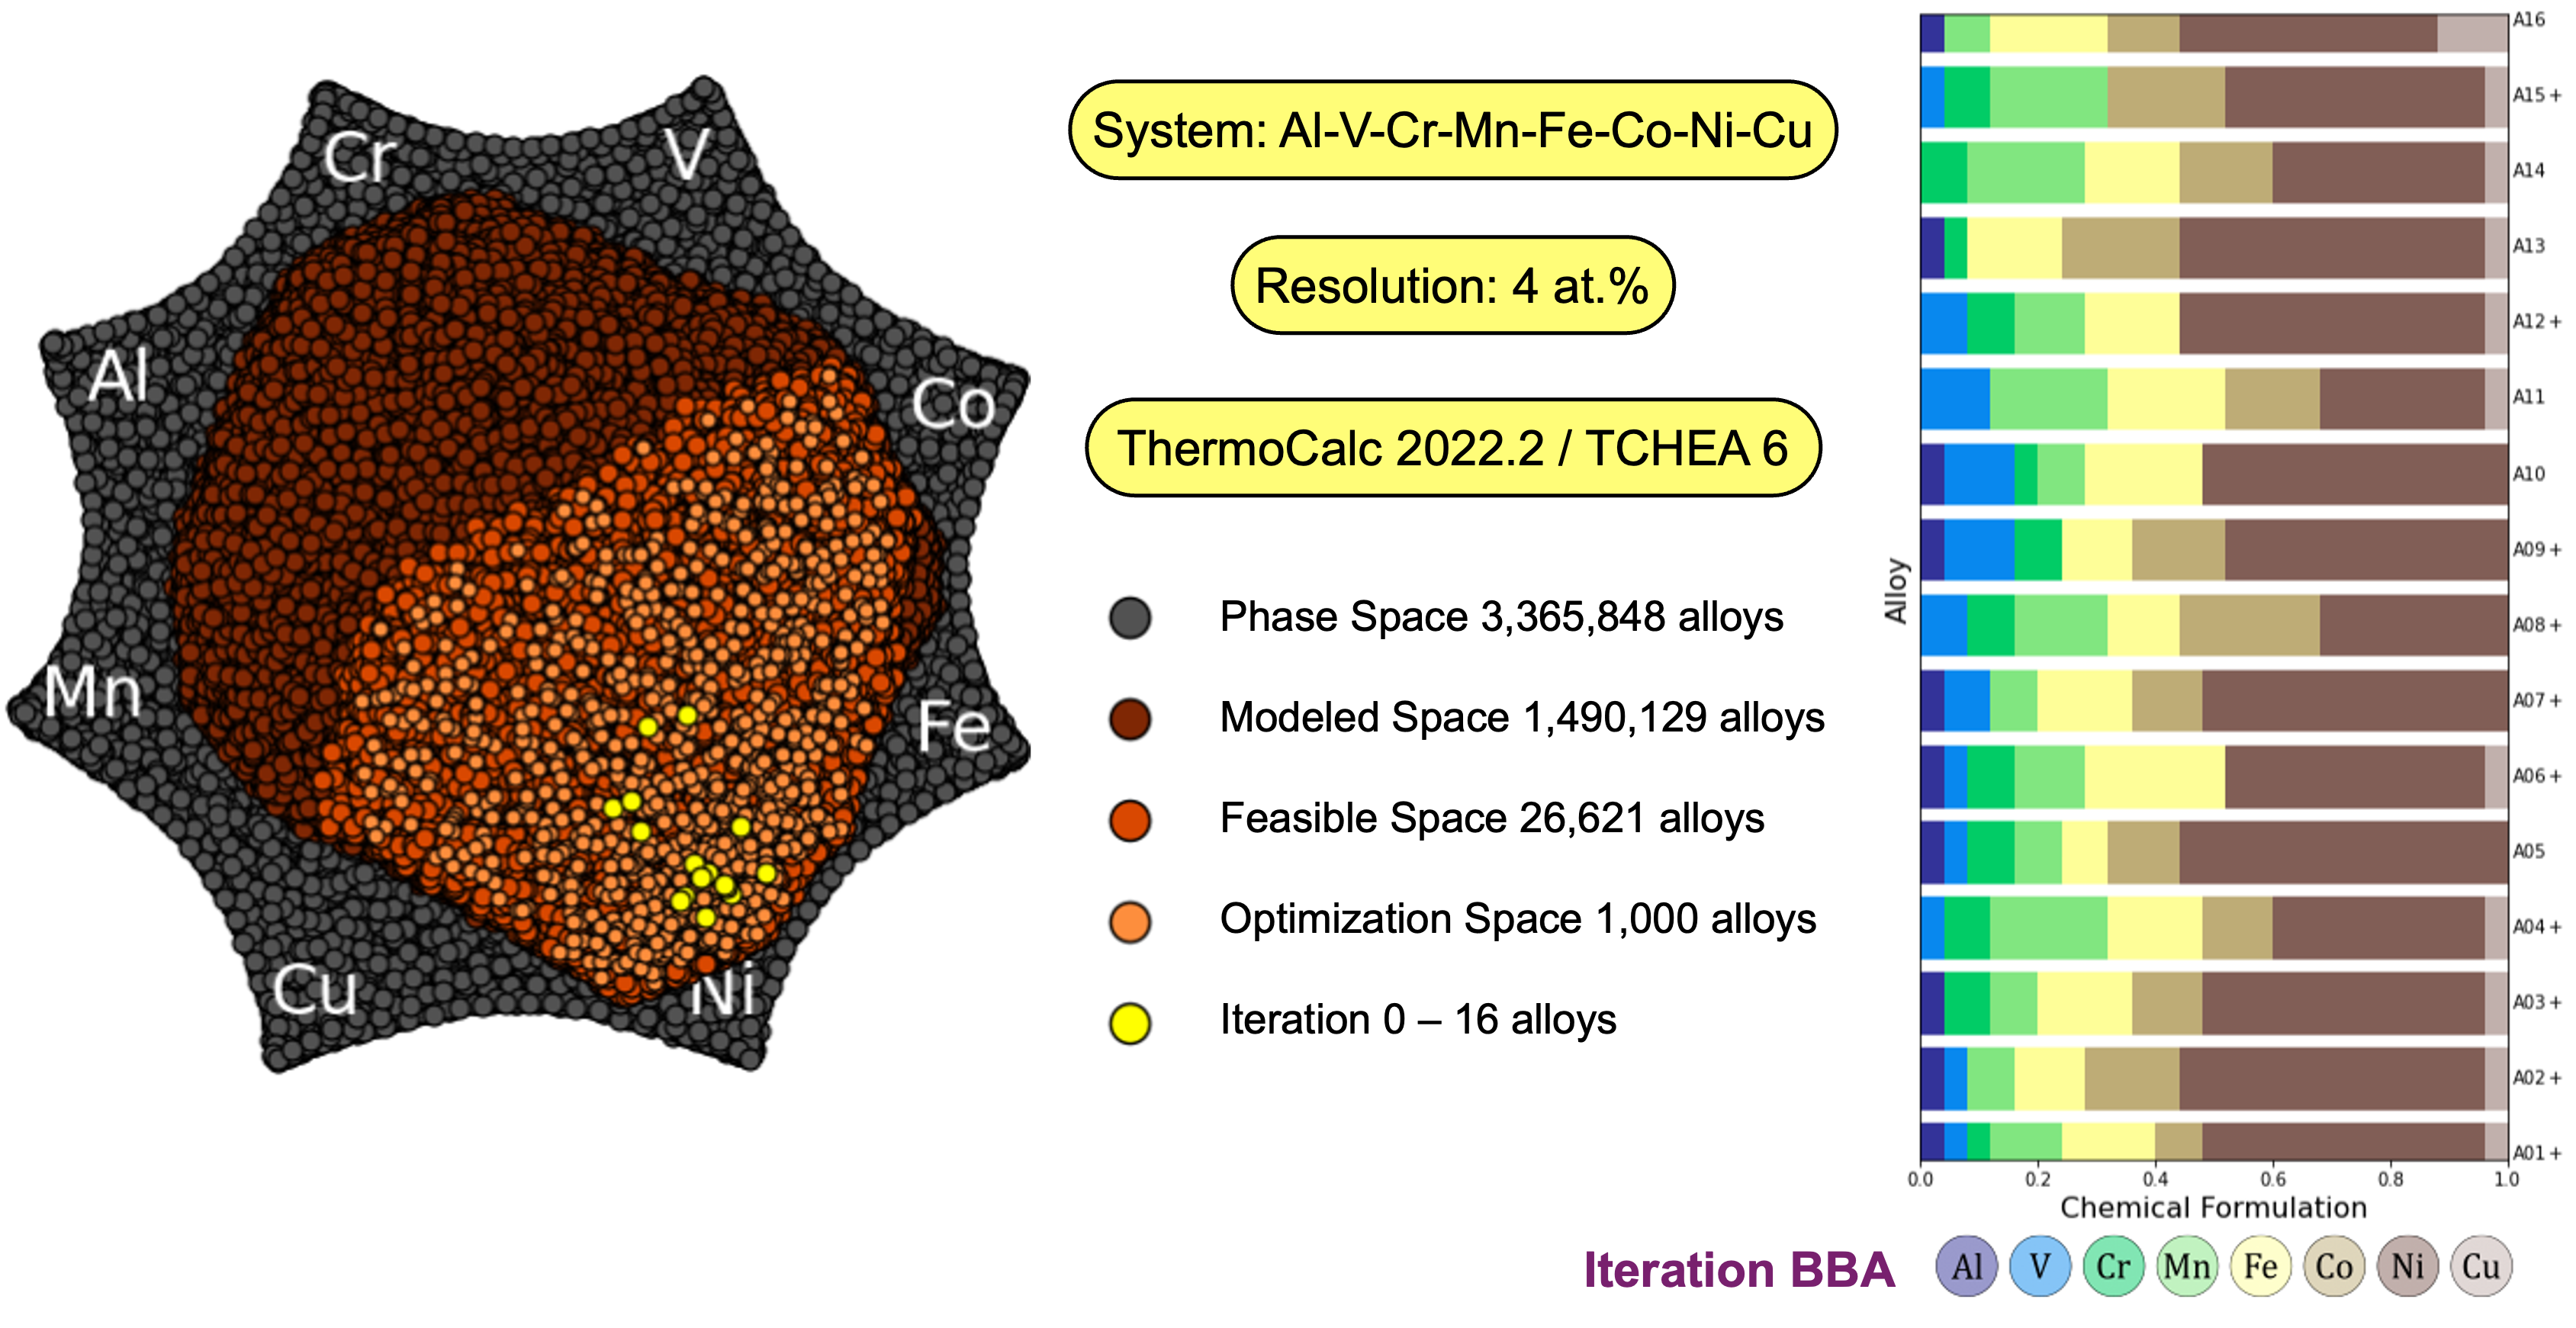
\includegraphics[width=0.8\columnwidth]{Figures/BBA_Suggestions_v2.png}
    \caption{Candidate alloy suggestions for Iteration 0 (BBA)}
    \label{fig:BBA}
\end{figure}

\subsubsection{Verification and Metallography}

All 16 candidate alloys synthesized in Iteration BBA were successfully fabricated using vacuum arc melting (VAM), followed by cold rolling and recrystallization annealing. The processing route produced dense, defect-free ingots with consistent surface quality and compositional uniformity. The alloys were subjected to a standardized high-throughput metallographic preparation pipeline to enable phase and microstructural verification prior to mechanical testing.

Phase stability and microstructural homogeneity of the processed candidate alloys, assessed using X-ray diffraction (XRD) confirmed the presence of face-centered cubic (FCC) structure in most alloys, consistent with the alloy design objectives. The FCC diffraction plots from across 3 iterations have been presented in \autoref{fig:Phase_Analysis} (a-c). Secondary intermetallic sigma ($P4_{2}/mnm$) type phase, present in some selective alloys 
from Iterations 2 and 3, have additionally been shown in \autoref{fig:Phase_Analysis}.

%Backscattered electron (BSE) imaging in scanning electron microscopy (SEM) confirmed the absence of macroscopic segregation, porosity, or inclusions in the majority of samples. Electron backscatter diffraction (EBSD) analysis revealed recrystallized, equiaxed microstructures with average grain sizes ranging from ~10µm to 35µm, a representative alloy is shown in \autoref{fig:BSE_SEM}. The more compositionally complex alloys (containing 7–8 elements) generally showed finer grains and narrower distributions, consistent with known sluggish diffusion effects in high entropy systems. Inverse pole figure (IPF) maps demonstrated largely random texture across all samples, indicating that recrystallization had effectively reset any deformation-induced orientation bias introduced during cold rolling.

\begin{figure}[H]
    \centering
    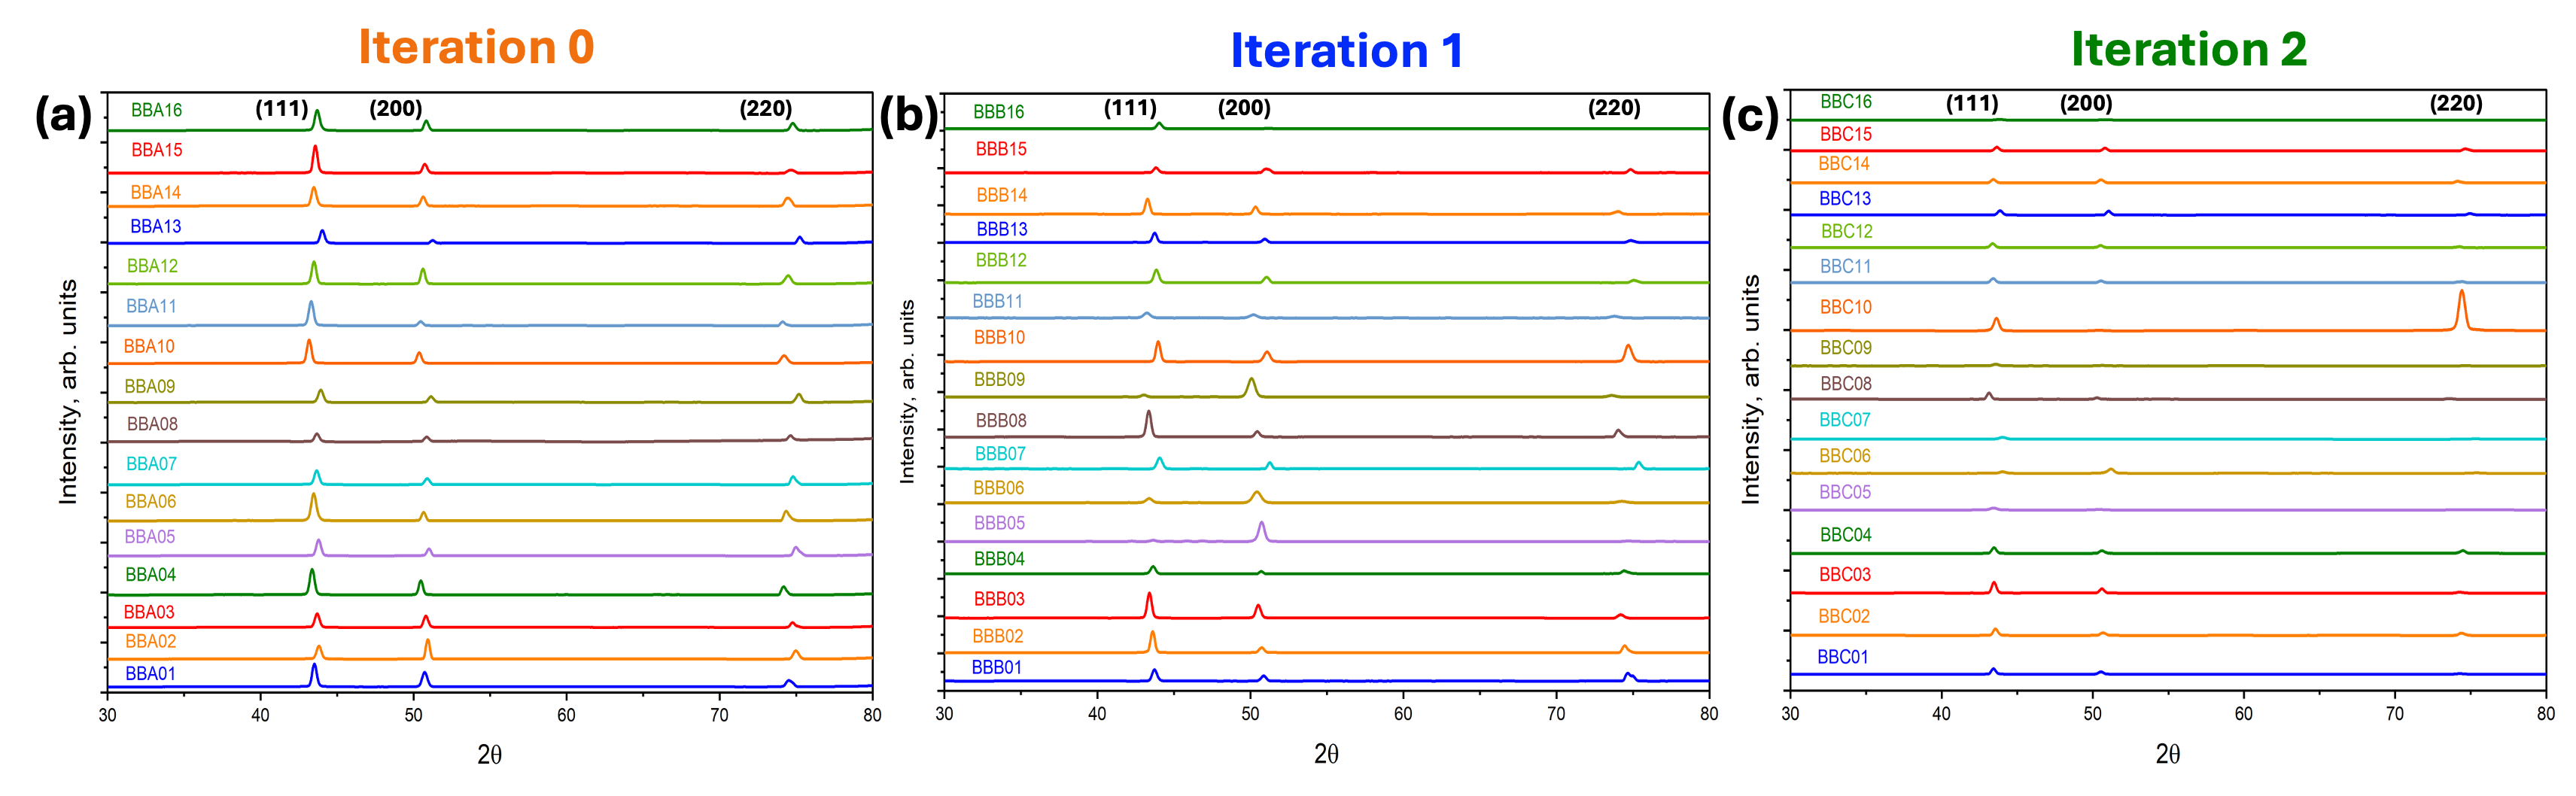
\includegraphics[width=0.9\columnwidth]{Figures/phase_analysis_C2.png}
    \caption{X-ray diffraction (XRD) patterns for all alloys across 3 iterations (a--c), representing specific FCC spectral peaks at (111), (200), and (220) planar reflections}
    \label{fig:Phase_Analysis}
\end{figure}

Sigma phase was observed to appear in alloys with high V + Cr content ($>$20~at.\%), although exception was found in several alloys (BBA09, BBB01, BBB03, BBC02, and BBC04). These alloys, however, had higher Ni content ($>$36~at.\%) that increased the Valence Electron Configuration (VEC), thus destabilizing secondary intermetallic phases. 

\autoref{fig:BSE_SEM}(a-c) presents BSE-SEM images of 3 selected specific alloy compositions, one from each iteration, revealing fully recrystallized polycrystalline equiaxed FCC grain structures with an abundance of annealing twins. Significant porosity and macrosegregation was absent in all inspected samples. The correspomding EBSD Inverse Pole Figure (IPF) maps, shown in \autoref{fig:BSE_SEM}(d-f) were used to analyze grain orientations and estimate approximate grain size (equivalent circle) distributions. IPF maps revealed absence of textural anisotropy, indicating that recrystallization heat treatments reset the preferential textures arising from cold rolling. The grain size distributions are summarized in \autoref{fig:BSE_SEM}(g–i) with descriptive statistics. For majority of the analyzed compositions, the average grain sizes ranged between 10~$\mu$m and 35~$\mu$m. The more compositionally complex alloys (possessing 7 to 8 elements) generally exhibited refined grains and narrower grain size distributions, consistent with the theories of sluggish diffusion in high entropy systems. 

\begin{figure}[hbt]
    \centering
    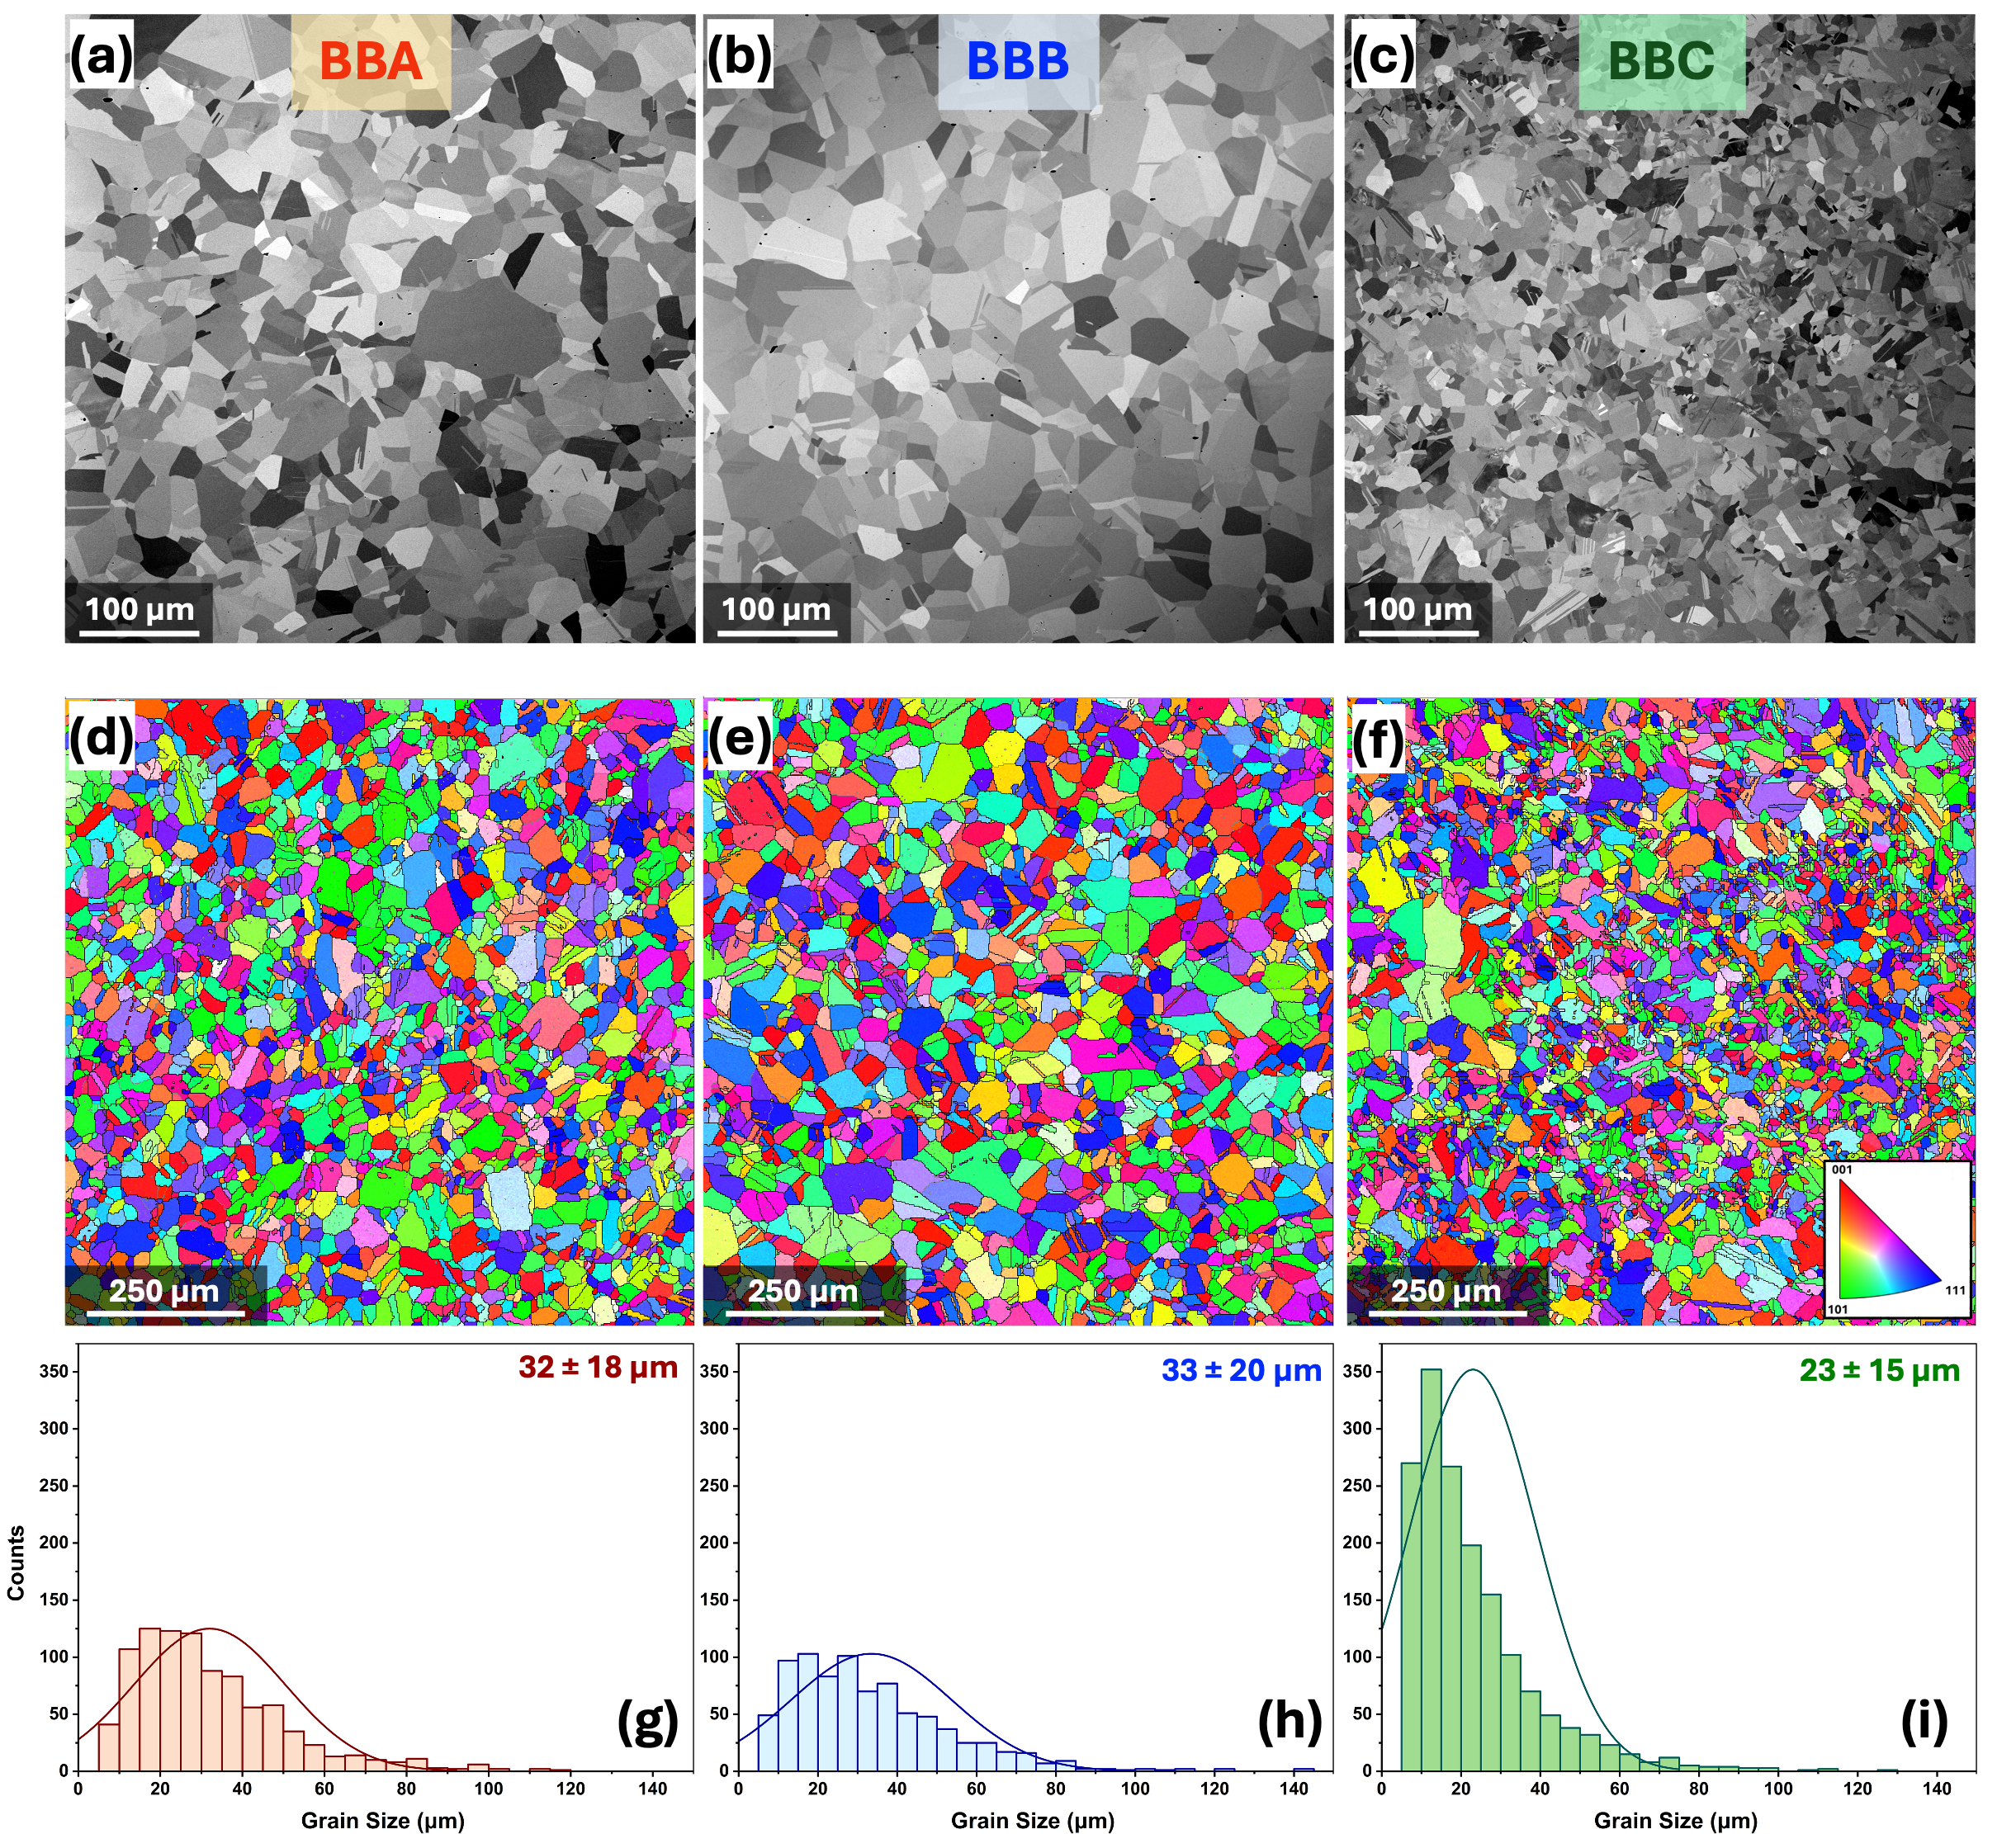
\includegraphics[width=0.7\columnwidth]{Figures/BSE_SEM_v3.png}
    \caption{Microstructure of selective FCC alloy compositions across 3 distinct iterations (a--c) SEM-BSE micrographs revealing fully recrystallized equiaxed FCC grains, (d--f) corresponding EBSD IPF maps exhibiting overall random textures across the polycrystalline materials, and (g--i) grain size histograms under normal distributions acquired from the corresponding EBSD dataset. Mean grain sizes across all materials range between $\sim$15~$\mu$m to 35~$\mu$m. }
    \label{fig:BSE_SEM}
\end{figure}

%The microstructural uniformity and phase stability were further verified by X-ray diffraction (XRD). All 16 synthesized alloys from Iteration BBA were validated as fully FCC through X-ray Diffraction (XRD) analysis shown in \autoref{fig:Phase_Analysis}. These results validated the initial CALPHAD predictions generated using the TCHEA6 database at 700°C and demonstrated the reliability of the VAM + thermomechanical processing route for producing structurally sound, phase-pure alloys. 

Alloys possessing homogeneous FCC microstructure were consequently subjected to mechanical testing. Some of the predicted alloys possessed brittle intermetallic Sigma phase, which were generally rich in Cr and V. Those alloys were labelled as brittle, and although, had passed the initial screening phase, did not survive the processing and mechanical testing stages due to localized cracking or premature failures under tensile tests.     

%Alloys with clean, homogeneous microstructure proceeded to full mechanical characterization, while those showing anomalies violating the design constraints, such as secondary precipitation or localized cracking during sample preparation were flagged for additional evaluation. These observations were critical for identifying potentially brittle alloys that may have passed initial phase screening but failed under mechanical or metallographic stresses. 


Below is the list of target composition of candidate alloys across three iterations in this study, composition measured by EDS analysis and XRD phase verification tabulated by iteration (\autoref{table_bba}, \autoref{table_bbb}, \autoref{table_bbc}). Candidates which violated project constraints, highlighted in red, had either manufacturing issues or secondary phases and were not characterized with EDS. These outcomes were used to inform the Bayesian optimization loop and retrain the feasibility classifier guiding future acquisition. Following complete characterization of candidate alloys from each iteration, the next batch of 16 candidate alloys was selected using the Bayesian optimization framework, which incorporated mechanical property feedback from previous iterations.

% \paragraph{BBA Alloys}
\begin{table}[H]
\caption{Composition and phase analysis of BBA (Iteration 0) alloys}
\label{table_bba}
\centering
\footnotesize
\resizebox{0.9\textwidth}{!}{
\begin{tblr}{
    hlines,
    hline{3,21} = {2pt},
    rowsep=1pt,
    colspec = {
        |X[1.2, c]
        |[2pt]X[0.7, c]|X[0.7, c]|X[0.7, c]|X[0.7, c]|X[0.7, c]|X[0.7, c]|X[0.7, c]|X[0.7, c]
        |[2pt]X[0.7, c]|X[0.7, c]|X[0.7, c]|X[0.7, c]|X[0.7, c]|X[0.7, c]|X[0.7, c]|X[0.7, c]
        |[2pt]X[2.0, c]
        |X[2.0, c]|
        },
    colsep=0pt,
    }
    \SetCell[r=2,c=1]{c}\textbf{\makecell{Alloy\\Name}}
    & \SetCell[c=8]{c} \textbf{Target Atomic \%}
    &&&&&&&& \SetCell[c=8]{c} \textbf{EDS Measured Atomic \%}
    &&&&&&&& \SetCell[r=2,c=1]{c}\textbf{XRD Phase} \\  
    & Al & Co & Cr & Cu & Fe & Mn & Ni & V
    & Al & Co & Cr & Cu & Fe & Mn & Ni & V \\
    BBA01 & 4 & 8 & 4 & 4 & 16 & 12 & 48 & 4 & 4.1 & 8.2 & 4.2 & 4.2 & 16.1 & 12.2 & 47.0 & 4.1 & FCC \\
    BBA02 & 4 & 16 & \SetCell{gray!20}0 & 4 & 12 & 8 & 52 & 4 & 4.2 & 15.0 & \SetCell{gray!20}0.0 & 4.2 & 12.2 & 8.2 & 52.2 & 4.1 & FCC \\
    BBA03 & 4 & 12 & 8 & 4 & 16 & 8 & 48 & \SetCell{gray!20}0 & 4.3 & 12.1 & 8.2 & 4.2 & 16.1 & 8.2 & 47.0 & \SetCell{gray!20}0.0 & FCC \\
    \SetCell{red!20}\textbf{BBA04} & \SetCell{gray!20}0 & 12 & 8 & 4 & 16 & 20 & 36 & 4 & $\cdot$ & $\cdot$ & $\cdot$ & $\cdot$ & $\cdot$ & $\cdot$ & $\cdot$ & $\cdot$ & \SetCell{red!20}\textbf{---} \\
    BBA05 & 4 & 12 & 8 & \SetCell{gray!20}0 & 8 & 8 & 56 & 4 & 4.1 & 12.2 & 8.2 & \SetCell{gray!20}0.0 & 8.2 & 8.0 & 55.2 & 4.1 & FCC \\
    BBA06 & 4 & \SetCell{gray!20}0 & 8 & 4 & 24 & 12 & 44 & 4 & 4.2 & \SetCell{gray!20}0.0 & 8.3 & 4.1 & 24.0 & 11.9 & 43.4 & 4.1 & FCC \\
    BBA07 & 4 & 12 & \SetCell{gray!20}0 & \SetCell{gray!20}0 & 16 & 8 & 52 & 8 & 5.0 & 12.3 & \SetCell{gray!20}0.0 & \SetCell{gray!20}0.0 & 16.2 & 7.9 & 50.5 & 8.1 & FCC \\
    BBA08 & \SetCell{gray!20}0 & 24 & 8 & \SetCell{gray!20}0 & 12 & 16 & 32 & 8 & \SetCell{gray!20}0.0 & 22.9 & 8.1 & \SetCell{gray!20}0.0 & 12.2 & 16.0 & 32.7 & 8.1 & FCC \\
    BBA09 & 4 & 16 & 8 & \SetCell{gray!20}0 & 12 & \SetCell{gray!20}0 & 48 & 12 & 4.9 & 16.1 & 8.2 & \SetCell{gray!20}0.0 & 12.0 & \SetCell{gray!20}0.0 & 46.6 & 12.1 & FCC \\
    BBA10 & 4 & \SetCell{gray!20}0 & 4 & \SetCell{gray!20}0 & 20 & 8 & 52 & 12 & 4.4 & \SetCell{gray!20}0.0 & 4.2 & \SetCell{gray!20}0.0 & 20.2 & 8.0 & 51.0 & 12.2 & FCC \\
    BBA11 & \SetCell{gray!20}0 & 16 & \SetCell{gray!20}0 & 4 & 20 & 20 & 28 & 12 & \SetCell{gray!20}0.0 & 16.1 & \SetCell{gray!20}0.0 & 4.0 & 20.1 & 20.3 & 27.4 & 12.0 & FCC \\
    BBA12 & \SetCell{gray!20}0 & \SetCell{gray!20}0 & 8 & 4 & 16 & 12 & 52 & 8 & \SetCell{gray!20}0.0 & \SetCell{gray!20}0.0 & 8.3 & 4.1 & 16.1 & 12.3 & 51.2 & 8.0 & FCC \\
    BBA13 & 4 & 20 & 4 & 4 & 16 & \SetCell{gray!20}0 & 52 & \SetCell{gray!20}0 & 4.0 & 20.4 & 4.1 & 4.2 & 16.3 & \SetCell{gray!20}0.0 & 51.0 & \SetCell{gray!20}0.0 & FCC \\
    BBA14 & \SetCell{gray!20}0 & 16 & 8 & 4 & 16 & 20 & 36 & \SetCell{gray!20}0 & \SetCell{gray!20}0.0 & 16.1 & 8.2 & 4.0 & 16.0 & 20.3 & 35.3 & \SetCell{gray!20}0.0 & FCC \\
    BBA15 & \SetCell{gray!20}0 & 20 & 8 & 4 & \SetCell{gray!20}0 & 20 & 44 & 4 & \SetCell{gray!20}0.0 & 19.9 & 8.2 & 4.2 & \SetCell{gray!20}0.0 & 20.5 & 43.2 & 4.0 & FCC \\
    BBA16 & 4 & 12 & \SetCell{gray!20}0 & 12 & 20 & 8 & 44 & \SetCell{gray!20}0 & 4.1 & 12.3 & \SetCell{gray!20}0.0 & 11.8 & 20.4 & 8.1 & 43.2 & \SetCell{gray!20}0.0 & FCC \\
\end{tblr}
}
\end{table}

% \paragraph{BBB Alloys}
\begin{table}[H]
\caption{Composition and phase analysis of BBB (Iteration 1) alloys}
\label{table_bbb}
\centering
\footnotesize
\resizebox{0.9\textwidth}{!}{
\begin{tblr}{
    hlines,
    hline{3,17} = {2pt},
    rowsep=1pt,
    colspec = {
        |X[1.2, c]
        |[2pt]X[0.7, c]|X[0.7, c]|X[0.7, c]|X[0.7, c]|X[0.7, c]|X[0.7, c]|X[0.7, c]|X[0.7, c]
        |[2pt]X[0.7, c]|X[0.7, c]|X[0.7, c]|X[0.7, c]|X[0.7, c]|X[0.7, c]|X[0.7, c]|X[0.7, c]
        |[2pt]X[2.0, c]
        |X[2.0, c]|
        },
    colsep=0pt,
    }
    \SetCell[r=2,c=1]{c}\textbf{\makecell{Alloy\\Name}}
    & \SetCell[c=8]{c} \textbf{Target Atomic \%}
    &&&&&&&& \SetCell[c=8]{c} \textbf{EDS Measured Atomic \%}
    &&&&&&&& \SetCell[r=2,c=1]{c}\textbf{XRD Phase} \\  
    & Al & Co & Cr & Cu & Fe & Mn & Ni & V
    & Al & Co & Cr & Cu & Fe & Mn & Ni & V \\
    BBB01 & \SetCell{gray!20}0 & 24 & 4 & \SetCell{gray!20}0 & 8 & 4 & 36 & 24 & \SetCell{gray!20}0.0 & 20.5 & 4.2 & \SetCell{gray!20}0.0 & 8.1 & 4.0 & 38.9 & 24.4 & FCC \\
    BBB02 & 4 & 32 & 8 & 4 & 4 & 20 & 24 & 4 & 4.2 & 30.4 & 8.2 & 4.1 & 4.1 & 20.1 & 24.7 & 4.1 & FCC \\
    BBB03 & 4 & \SetCell{gray!20}0 & 12 & 4 & 4 & 16 & 52 & 8 & 4.1 & $\cdot$ & 12.3 & 4.1 & 4.1 & 16.1 & 51.2 & 8.2 & FCC \\
    BBB04 & 4 & 12 & 4 & \SetCell{gray!20}0 & 28 & \SetCell{gray!20}0 & 40 & 12 & 4.0 & 11.1 & 4.1 & \SetCell{gray!20}0.0 & 28.0 & \SetCell{gray!20}0.0 & 40.8 & 12.0 & FCC \\
    \SetCell{red!20}\textbf{BBB05} & \SetCell{gray!20}0 & 44 & 12 & \SetCell{gray!20}0 & 4 & 4 & 12 & 24 & $\cdot$ & $\cdot$ & $\cdot$ & $\cdot$ & $\cdot$ & $\cdot$ & $\cdot$ & $\cdot$ & \SetCell{red!20}\textbf{$\mathbf{FCC+\sigma}$} \\
    \SetCell{red!20}\textbf{BBB06} & \SetCell{gray!20}0 & 16 & 20 & \SetCell{gray!20}0 & 4 & 4 & 36 & 20 & $\cdot$ & $\cdot$ & $\cdot$ & $\cdot$ & $\cdot$ & $\cdot$ & $\cdot$ & $\cdot$ & \SetCell{red!20}\textbf{$\mathbf{FCC+\sigma}$} \\
    BBB07 & 4 & 40 & \SetCell{gray!20}0 & \SetCell{gray!20}0 & 12 & 4 & 36 & 4 & 4.0 & 39.1 & \SetCell{gray!20}0.0 & \SetCell{gray!20}0.0 & 12.3 & 3.9 & 36.7 & 4.0 & FCC \\
    BBB08 & 4 & 8 & 12 & 4 & 4 & 24 & 40 & 4 & 3.8 & 8.0 & 12.3 & 4.2 & 4.1 & 24.0 & 39.4 & 4.1 & FCC \\
    \SetCell{red!20}\textbf{BBB09} & \SetCell{gray!20}0 & 4 & 8 & \SetCell{gray!20}0 & 4 & 28 & 40 & 16 & $\cdot$ & $\cdot$ & $\cdot$ & $\cdot$ & $\cdot$ & $\cdot$ & $\cdot$ & $\cdot$ & \SetCell{red!20}\textbf{$\mathbf{FCC+\sigma}$} \\
    BBB10 & 4 & \SetCell{gray!20}0 & 4 & 4 & 8 & 16 & 52 & 12 & $\cdot$ & $\cdot$ & $\cdot$ & $\cdot$ & $\cdot$ & $\cdot$ & $\cdot$ & $\cdot$ & FCC \\
    \SetCell{red!20}\textbf{BBB11} & \SetCell{gray!20}0 & 24 & 4 & \SetCell{gray!20}0 & 4 & 32 & 20 & 16 & $\cdot$ & $\cdot$ & $\cdot$ & $\cdot$ & $\cdot$ & $\cdot$ & $\cdot$ & $\cdot$ & \SetCell{red!20}\textbf{$\mathbf{FCC+\sigma}$} \\
    BBB12 & \SetCell{gray!20}0 & 20 & 4 & \SetCell{gray!20}0 & 4 & 4 & 48 & 20 & \SetCell{gray!20}0.0 & 20.2 & 4.2 & \SetCell{gray!20}0.0 & 4.1 & 4.0 & 47.1 & 20.4 & FCC \\
    \SetCell{red!20}\textbf{BBB13} & \SetCell{gray!20}0 & 40 & 4 & \SetCell{gray!20}0 & 28 & 4 & 4 & 20 & 0.0 & 39.7 & 4.2 & 0.0 & 27.9 & 3.9 & 4.2 & 20.1 & \SetCell{red!20}\textbf{$\mathbf{FCC+\sigma}$} \\
    BBB14 & 4 & \SetCell{gray!20}0 & 12 & 16 & 4 & 12 & 52 & \SetCell{gray!20}0 & 4.4 & \SetCell{gray!20}0.0 & 12.1 & 15.7 & 4.1 & 12.4 & 51.3 & \SetCell{gray!20}0.0 & FCC \\
    BBB15 & 4 & \SetCell{gray!20}0 & 8 & 24 & 4 & 16 & 44 & \SetCell{gray!20}0 & 4.3 & \SetCell{gray!20}0.0 & 8.3 & 23.5 & 4.1 & 16.2 & 43.7 & \SetCell{gray!20}0.0 & FCC \\
    BBB16 & 4 & 36 & \SetCell{gray!20}0 & \SetCell{gray!20}0 & 4 & 4 & 40 & 12 & $\cdot$ & $\cdot$ & $\cdot$ & $\cdot$ & $\cdot$ & $\cdot$ & $\cdot$ & $\cdot$ & FCC \\
\end{tblr}
}
\end{table}

% \paragraph{BBC Alloys}
\begin{table}[H]
\caption{Composition and phase analysis of BBC (Iteration 2) alloys}
\label{table_bbc}
\centering
\footnotesize
\resizebox{0.9\textwidth}{!}{
\begin{tblr}{
    hlines,
    hline{3,17} = {2pt},
    rowsep=1pt,
    colspec = {
        |X[1.2, c]
        |[2pt]X[0.7, c]|X[0.7, c]|X[0.7, c]|X[0.7, c]|X[0.7, c]|X[0.7, c]|X[0.7, c]|X[0.7, c]
        |[2pt]X[0.7, c]|X[0.7, c]|X[0.7, c]|X[0.7, c]|X[0.7, c]|X[0.7, c]|X[0.7, c]|X[0.7, c]
        |[2pt]X[2.0, c]
        |X[2.0, c]|
        },
    colsep=0pt,
    }
    \SetCell[r=2,c=1]{c}\textbf{\makecell{Alloy\\Name}}
    & \SetCell[c=8]{c} \textbf{Target Atomic \%}
    &&&&&&&& \SetCell[c=8]{c} \textbf{EDS Measured Atomic \%}
    &&&&&&&& \SetCell[r=2,c=1]{c}\textbf{XRD Phase} \\  
    & Al & Co & Cr & Cu & Fe & Mn & Ni & V
    & Al & Co & Cr & Cu & Fe & Mn & Ni & V \\
    BBC01 & 4 & 12 & 4 & 4 & 20 & 16 & 32 & 8 & 4.0 & 12.2 & 4.2 & 4.0 & 20.1 & 16.0 & 31.4 & 8.2 & FCC \\
    BBC02 & 4 & 8 & \SetCell{gray!20}0 & \SetCell{gray!20}0 & 4 & 8 & 52 & 24 & 4.0 & 8.2 & \SetCell{gray!20}0.0 & \SetCell{gray!20}0.0 & 4.1 & 8.0 & 51.2 & 24.4 & FCC \\
    \SetCell{red!20}\textbf{BBC03} & 4 & 4 & 12 & \SetCell{gray!20}0 & \SetCell{gray!20}0 & 4 & 52 & 24 & 4.0 & 4.1 & 12.2 & \SetCell{gray!20}0.0 & \SetCell{gray!20}0.0 & 3.9 & 51.3 & 24.4 & \SetCell{red!20}\textbf{$\mathbf{FCC+\sigma}$} \\
    BBC04 & 4 & \SetCell{gray!20}0 & 4 & \SetCell{gray!20}0 & 4 & 4 & 60 & 24 & 4.0 & \SetCell{gray!20}0.0 & 4.2 & \SetCell{gray!20}0.0 & 4.1 & 4.0 & 59.3 & 24.5 & FCC \\
    \SetCell{red!20}\textbf{BBC05} & \SetCell{gray!20}0 & 24 & 8 & \SetCell{gray!20}0 & 16 & 40 & 4 & 8 & $\cdot$ & $\cdot$ & $\cdot$ & $\cdot$ & $\cdot$ & $\cdot$ & $\cdot$ & $\cdot$ & \SetCell{red!20}\textbf{---} \\
    \SetCell{red!20}\textbf{BBC06} & 4 & 28 & 4 & \SetCell{gray!20}0 & 4 & 4 & 44 & 12 & $\cdot$ & $\cdot$ & $\cdot$ & $\cdot$ & $\cdot$ & $\cdot$ & $\cdot$ & $\cdot$ & \SetCell{red!20}\textbf{---} \\
    \SetCell{red!20}\textbf{BBC07} & 4 & 32 & 4 & \SetCell{gray!20}0 & \SetCell{gray!20}0 & 4 & 44 & 12 & $\cdot$ & $\cdot$ & $\cdot$ & $\cdot$ & $\cdot$ & $\cdot$ & $\cdot$ & $\cdot$ & \SetCell{red!20}\textbf{---} \\
    \SetCell{red!20}\textbf{BBC08} & \SetCell{gray!20}0 & 8 & \SetCell{gray!20}0 & 4 & 4 & 28 & 36 & 20 & $\cdot$ & 8.1 & $\cdot$ & 4.1 & 4.2 & 28.1 & 35.7 & 19.9 & \SetCell{red!20}\textbf{$\mathbf{FCC+\sigma}$} \\
    \SetCell{red!20}\textbf{BBC09} & \SetCell{gray!20}0 & 36 & 4 & \SetCell{gray!20}0 & 16 & 16 & 8 & 20 & $\cdot$ & $\cdot$ & $\cdot$ & $\cdot$ & $\cdot$ & $\cdot$ & $\cdot$ & $\cdot$ & \SetCell{red!20}\textbf{---} \\
    \SetCell{red!20}\textbf{BBC10} & 4 & 4 & 16 & \SetCell{gray!20}0 & 8 & \SetCell{gray!20}0 & 52 & 16 & $\cdot$ & $\cdot$ & $\cdot$ & $\cdot$ & $\cdot$ & $\cdot$ & $\cdot$ & $\cdot$ & \SetCell{red!20}\textbf{---} \\
    BBC11 & 4 & 12 & 4 & 4 & 12 & 16 & 36 & 12 & 4.3 & 12.2 & 4.2 & 3.9 & 12.2 & 15.9 & 35.1 & 12.3 & FCC \\
    BBC12 & 4 & 4 & 4 & 8 & 28 & 16 & 32 & 4 & 4.1 & 4.3 & 4.2 & 7.8 & 28.0 & 16.1 & 31.3 & 4.1 & FCC \\
    BBC13 & 4 & 28 & \SetCell{gray!20}0 & 20 & 4 & 8 & 36 & \SetCell{gray!20}0 & 4.3 & 28.0 & $\cdot$ & 19.9 & 4.1 & 8.4 & 35.4 & $\cdot$ & FCC \\
    \SetCell{red!20}\textbf{BBC14} & \SetCell{gray!20}0 & 12 & 4 & \SetCell{gray!20}0 & 4 & 16 & 40 & 24 & $\cdot$ & 12.1 & 4.1 & $\cdot$ & 4.3 & 16.1 & 39.0 & 24.5 & \SetCell{red!20}\textbf{$\mathbf{FCC+\sigma}$} \\
    BBC15 & 4 & 16 & \SetCell{gray!20}0 & 20 & 4 & 12 & 44 & \SetCell{gray!20}0 & 4.4 & 16.2 & $\cdot$ & 19.7 & 4.2 & 12.3 & 43.3 & $\cdot$ & FCC \\
    \SetCell{red!20}\textbf{BBC16} & 4 & 28 & 4 & \SetCell{gray!20}0 & 8 & \SetCell{gray!20}0 & 40 & 16 & $\cdot$ & $\cdot$ & $\cdot$ & $\cdot$ & $\cdot$ & $\cdot$ & $\cdot$ & $\cdot$ & \SetCell{red!20}\textbf{---} \\
\end{tblr}
}
\end{table}


\subsubsection{Challenges with Secondary Phases and Phase Prediction Discrepancies}


%Following this, a second batch of 16 candidate alloys (Iteration BBB) was selected using the Bayesian optimization framework, which incorporated mechanical property feedback from BAA. 
As noted above, phase analysis of the BBB samples revealed the presence of SIGMA phase in 5 out of the 16 alloys, indicating limitations in the TCHEA6 database’s predictive accuracy, particularly at elevated temperatures where secondary phases may emerge.


During this phase of the study, Thermo-Calc released the updated TCHEA7 database, offering refined phase stability predictions, including for SIGMA, BCC, HCP, and liquid phases across more than 100 systems (details of phase stability updates are included in the Supplementary Information). To address observed phase prediction discrepancies, we re-evaluated the full set of \(\sim 1.49\) million filtered compositions using TCHEA7, adding an additional constraint of \(\text{FCC} \geq 0.99\) at \(950^\circ\text{C}\) (representative of recrystallization temperatures), alongside the existing \(700^\circ\text{C}\) requirement. This step was motivated by observations from prior work, in which several alloys exhibited phase transformations or secondary FCC L1\(_2\) ordering at elevated temperatures.

This reanalysis with TCHEA7 led to both the removal of previously accepted candidates and the inclusion of new ones. Comparing TCHEA7 predictions with experimental XRD results for Iterations BBA and BBB revealed both false positives (predictions of secondary phases not observed experimentally), and false negatives (compositions predicted to be stable FCC that exhibited secondary phases in reality). At \(700^\circ\text{C}\), five false positives and two false negatives were recorded; at \(950^\circ\text{C}\), there was one false positive and four false negatives. False negatives are particularly problematic as they introduce the risk of synthesizing brittle or phase-unstable alloys.

To mitigate these risks, we adopted a more conservative constraint: only alloys predicted to be FCC-stable at both \(700^\circ\text{C}\) and \(950^\circ\text{C}\) were retained in the updated feasible set. This strategy yielded 27,240 alloys that met both phase stability criteria using TCHEA7, ensuring higher fidelity in downstream candidate selection. This refined feasible space now served as input to our Bayesian optimization framework, increasing confidence in the structural phase behavior of the alloys proposed in subsequent experimental iterations.


\subsection{Mechanical Characterization}
The mechanical properties of the candidate alloys in current study were evaluated using a suite of complementary testing methods designed to capture performance across a broad range of strain rates and deformation scales. Each alloy that passed microstructural verification proceeded through a standardized mechanical characterization workflow comprising quasistatic uniaxial tension, instrumented nanoindentation (NI), high strain rate nanoindentation (HSRNI), and split Hopkinson pressure bar (SHPB) testing, discussed in detail in Methods. %This multimodal strategy ensured a comprehensive assessment of strength, ductility, and dynamic behavior, key inputs to the multi-objective Bayesian optimization framework.


\subsubsection{Tension testing}


Quasi-static tensile tests reveal baseline mechanical performances of all alloys across 3 iterations. \autoref{fig:true_stress_strain} represents the true stress versus true strain curves, highlighting each alloy’s tensile performance. The true fracture stress mostly increased progressively across successive design iterations, while ductility remained comparable. The calculated values of YS, UTS, and strain to failure for all the tested alloys are mentioned in the SI. Tensile curves report progressive increase in true fracture stresses across iterations, with majority of the alloys surpassing 1 GPa in true tensile strength. 


\begin{figure}[H]
\centering
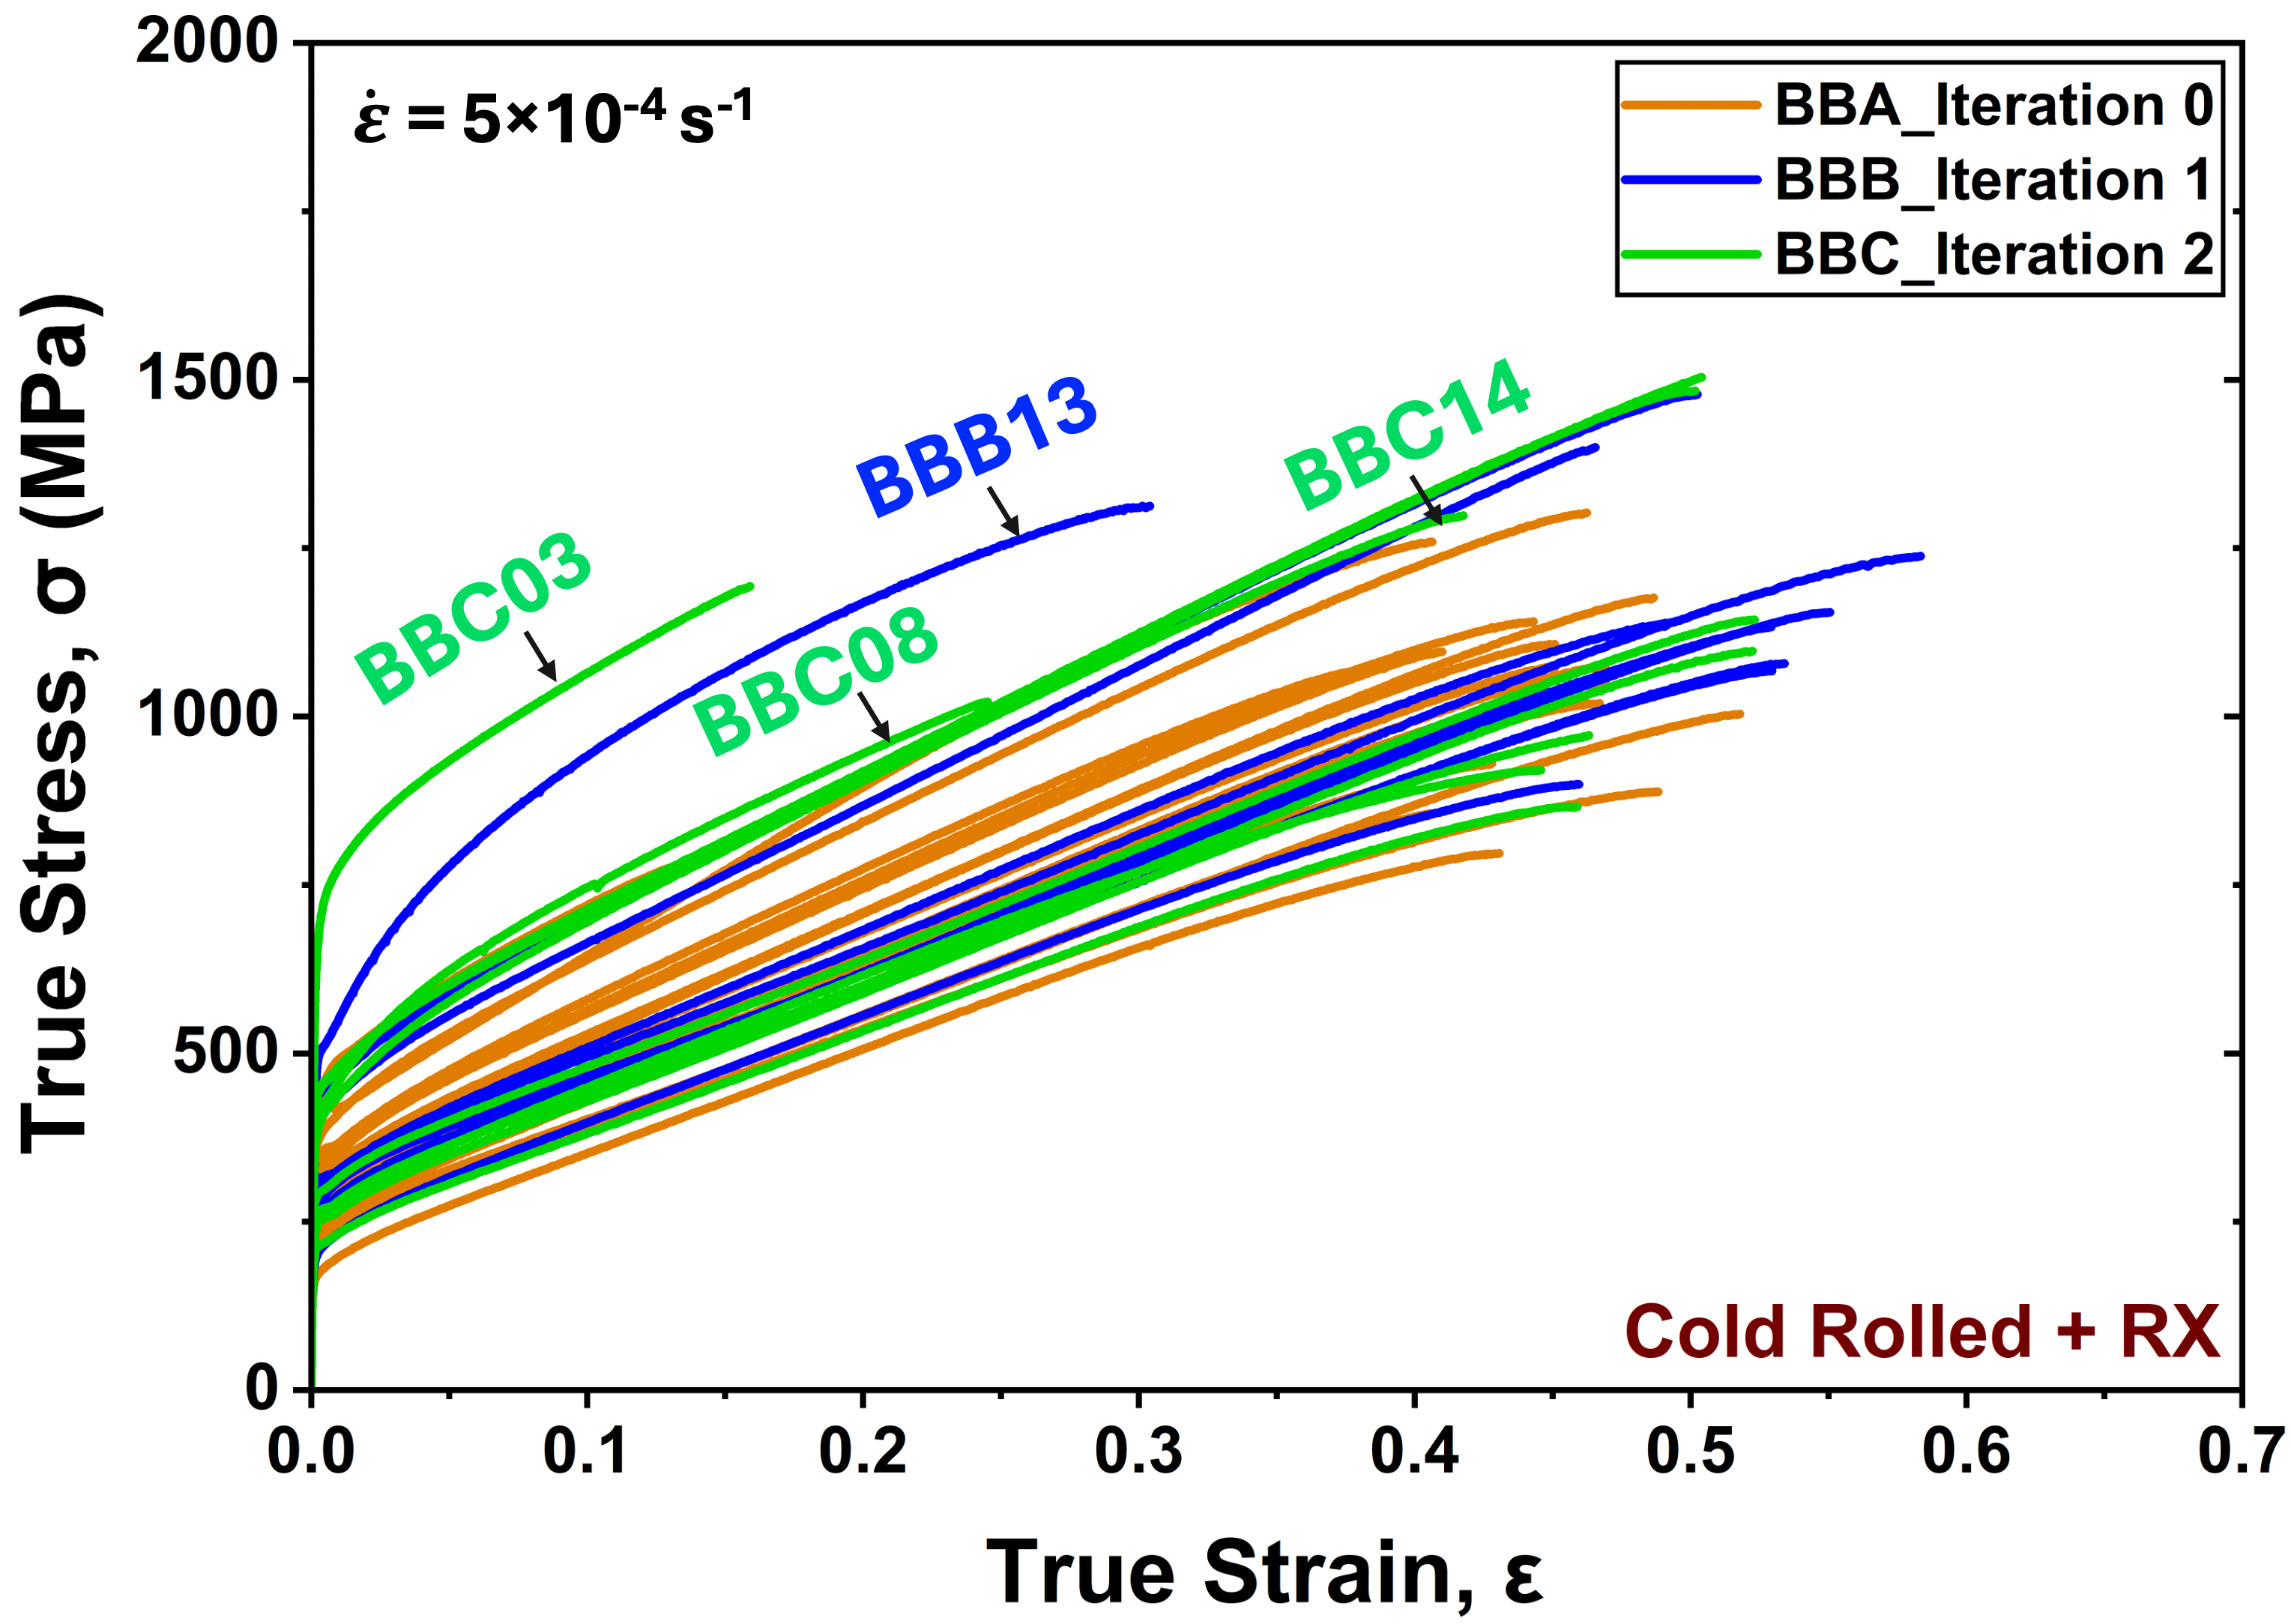
\includegraphics[width=0.5\linewidth]{Figures/Tension_BBA_BBB_BBC.png}
\caption{Consolidated true stress-strain curves acquired from ambient temperature quasistatic uniaxial tensile tests for tested FCC alloys across 3 iterations. Samples exhibiting sigma phase have been indicated by black arrows. RX refers to recrystallized alloys.}
\label{fig:true_stress_strain}
\end{figure}


Enhanced strain hardening was observed across iterations which delayed the onset of strain localizations, manifesting as a high UTS/YS ratio. Most importantly, these enhancements in strength levels was achieved without a significant reduction in ductility, as evidenced by sustained strain at UTS in the range of 45–50\% for top-performing (strongest) alloys. These improvements highlight the effectiveness of the Bayesian optimization loop in identifying alloy chemistries that balance strength with ductility, an essential trade-off in the development of materials for structural applications. Compositions exhibiting elevated UTS/YS ratios ($>$ 1.3) additionally demonstrated superior strain hardening behaviors, contributing to enhanced toughness and delayed failures under quasi-static regimes.

%Quasi-static tensile testing to evaluate baseline mechanical performance under low-rate loading conditions for all candidate alloys extracted the true stress–strain curves included yield strength (YS), ultimate tensile strength (UTS), UTS/YS ratio, and engineering strain at UTS. \autoref{fig:true_stress_strain} presents true stress versus true plastic strain curves for candidate alloys across all iterations. The curves show a progressive increase in true fracture stress across iterations, with several alloys from BBB surpassing 1.1 GPa in true tensile strength. Importantly, these gains in strength were achieved without significant reduction in ductility, as evidenced by sustained strain at UTS in the range of 5–9\% for top-performing alloys.

The extracted tensile properties from these curves, including yield strength (YS), UTS/YS ratio, and strain at UTS ($\varepsilon$), form 3 of the 5 key objectives in this Bayesian optimization framework. This data directly influences surrogate model training and informs the acquisition of candidates across subsequent design iterations.

%This improvement highlights the effectiveness of the Bayesian optimization loop in identifying alloy chemistries that balance strength with ductility, an essential trade-off in the development of materials for structural applications. Compositions exhibiting elevated UTS/YS ratios ($>$1.3) also demonstrated superior strain hardening behavior, contributing to enhanced toughness and delayed failure.

\subsubsection{High Strain Rate Nanoindentation Testing}

The nanoindentation testing revealed consistent differences between dynamic and quasi-static mechanical responses across all investigated high entropy alloy compositions. \autoref{fig:HSRNI1} presents the comparative hardness measurements for both loading conditions. In all samples, dynamic hardness values exceeded their quasi-static counterparts. This observation is consistent with the higher strain rate associated with dynamic loading conditions (\(\sim 10^3\,\text{s}^{-1}\)) relative to quasi-static testing (\(\sim 10^0\,\text{s}^{-1}\)).

\begin{figure}[hbt]
    \centering
    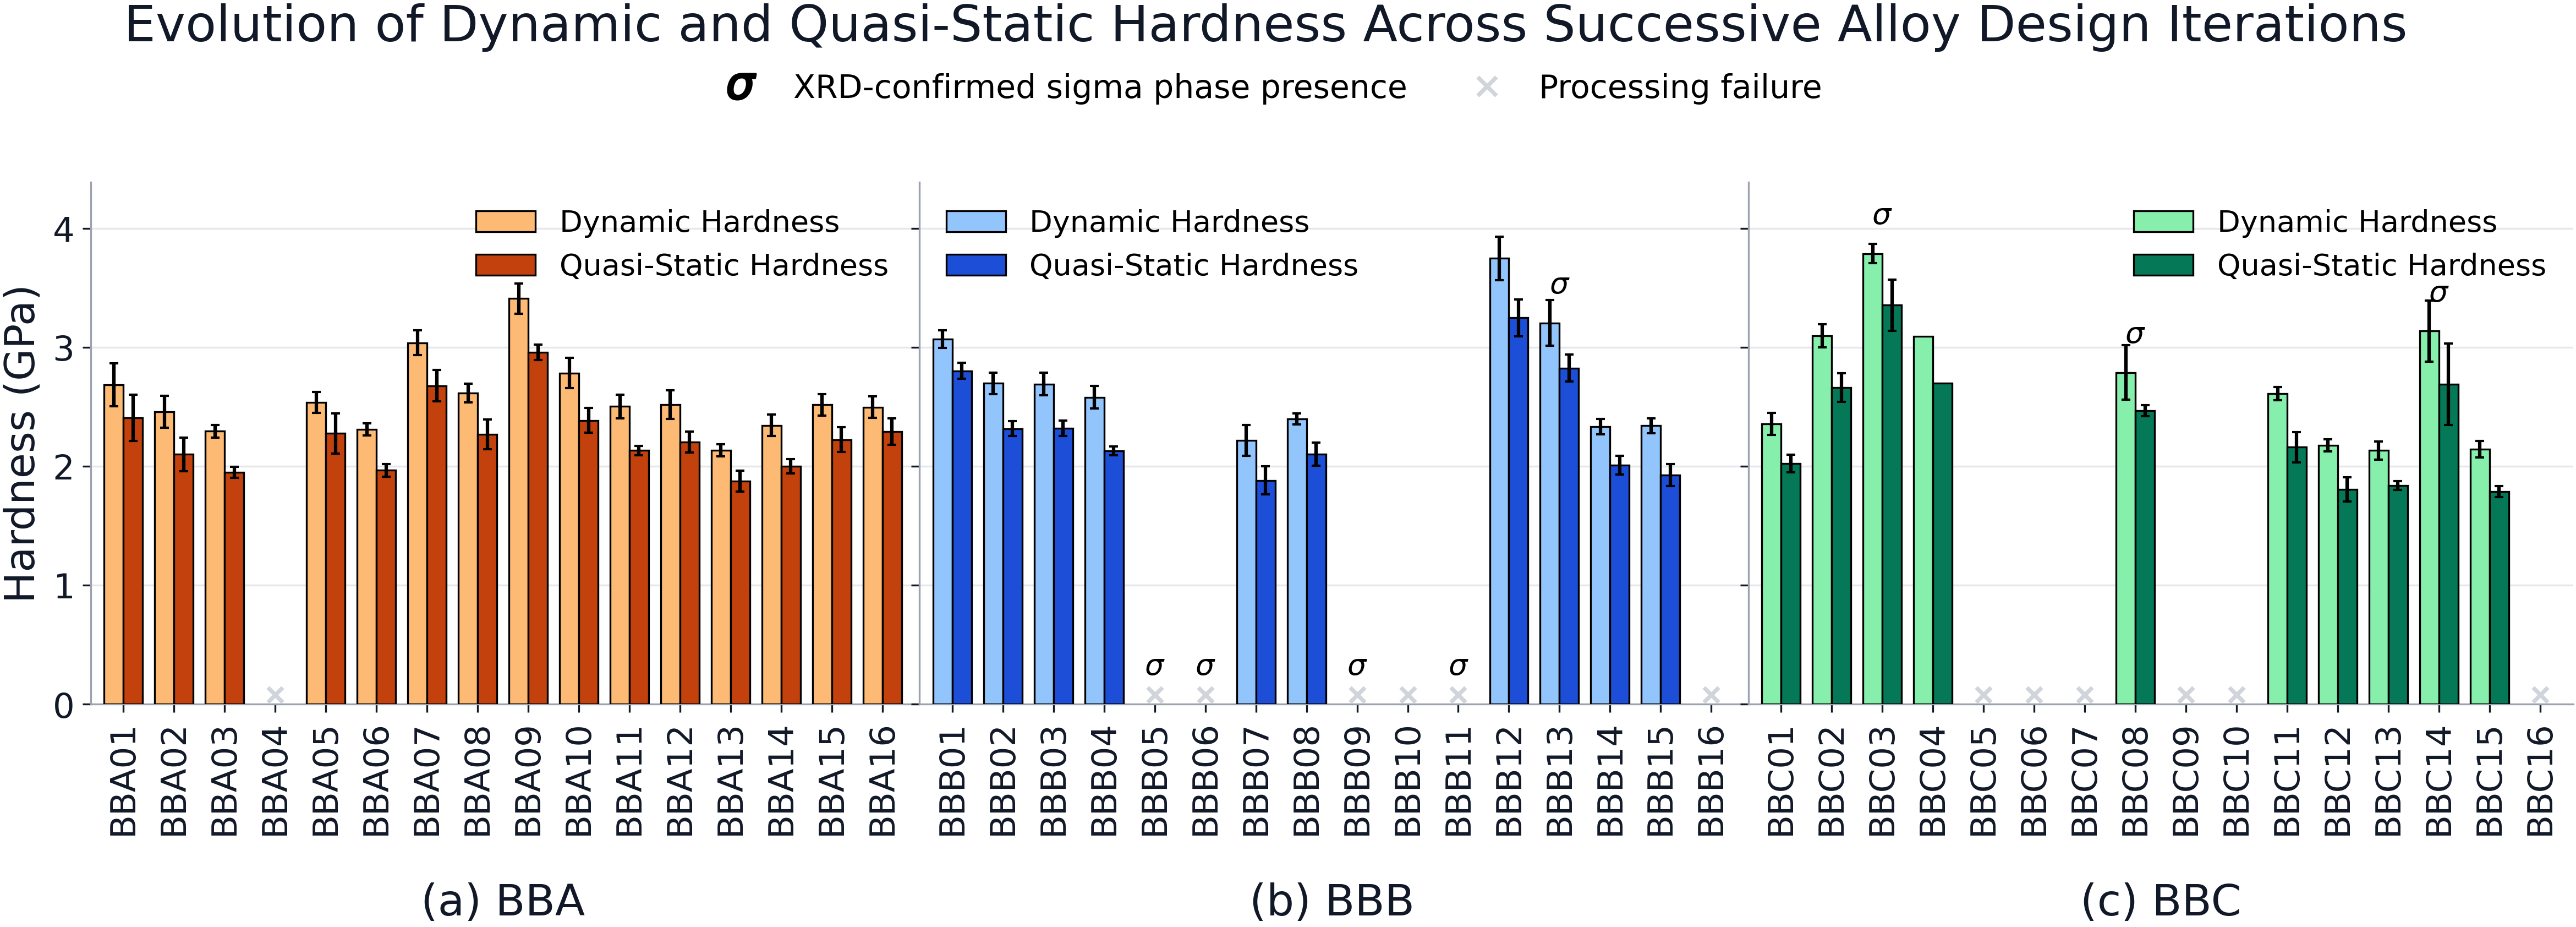
\includegraphics[width=0.9\columnwidth]{Figures/Hdyn_Hqs_1_02.png}
    \caption{Dynamic (blue) and Quasistatic (orange) hardness values as obtained from indentation constant strain rate tests and indentation impact tests. Results shown are for iteration (a) BBA, (b) BBB, and (c) BBC.}
    \label{fig:HSRNI1}
\end{figure}

Despite point-to-point scatter in the data, clear trends were observed. Sample \texttt{BBB12}, which exhibited a pure FCC microstructure, showed the highest hardness among the single-phase samples. Sample \texttt{BBC03} showed the overall highest hardness, which had confirmed presence of a secondary \(\sigma\) phase.

\emph{Dynamic to Quasi-static Hardness Ratio Analysis:} The dynamic to quasi-static hardness ratio, \(H_{\text{DYN}}/H_{\text{QS}}\), shown in \autoref{fig:HSRNI2}, ranged from 1.05 to 1.20 across all samples. No clear compositional trends were evident in the hardness ratio values across the study. These ratios were calculated using the average values of the measured hardnesses under both loading conditions. Error bars in the figure were computed via propagation of uncertainty from the standard deviations of both dynamic and quasi-static measurements. None of the tested compositions exhibited error bars that overlapped with a unity ratio, indicating a measurable difference between dynamic and quasi-static hardness in each case.

\begin{figure}[H]
    \centering
    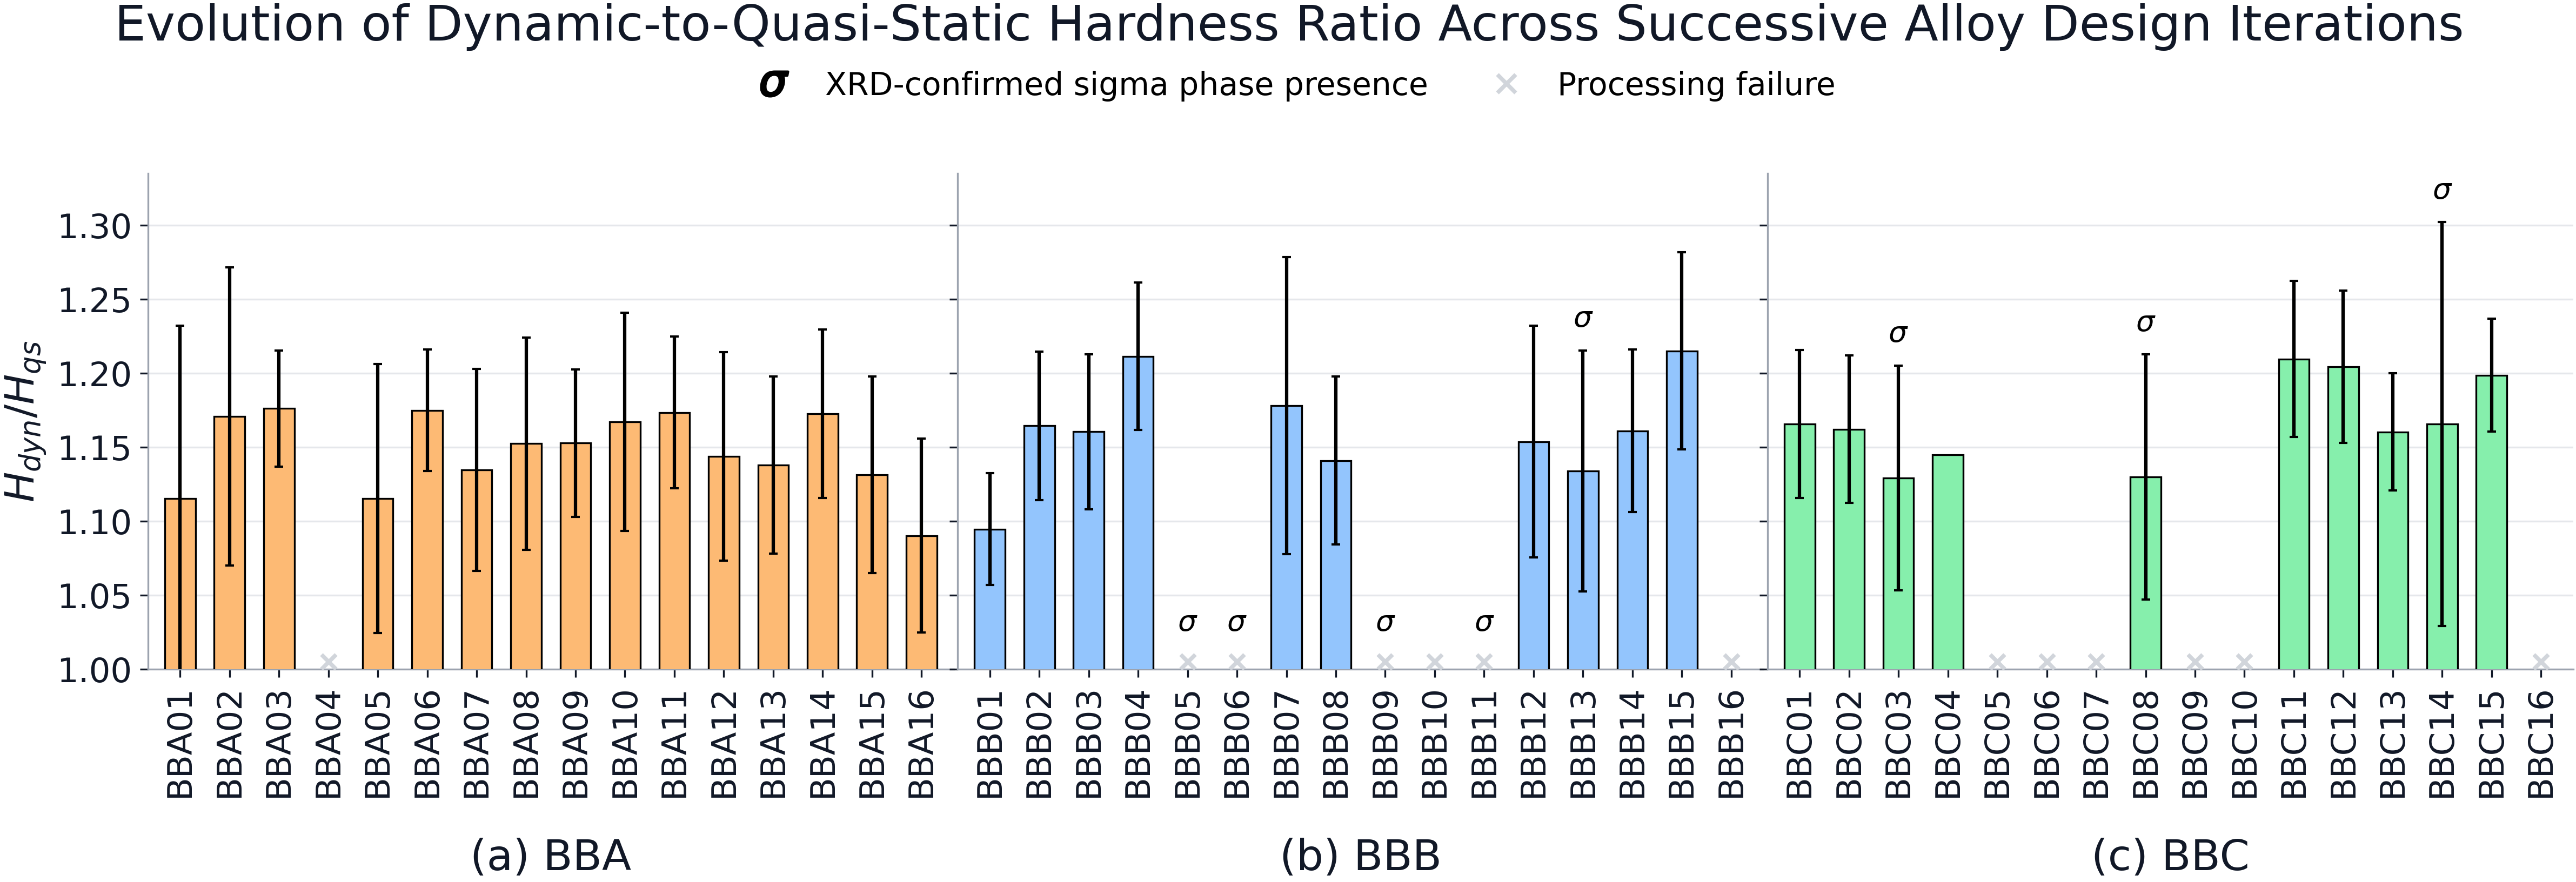
\includegraphics[width=0.9\columnwidth]{Figures/Dyn_QS_ratio_1.png}
    \caption{Calculated dynamic to quasistatic hardness ratio for (a) BBA, (b) BBB, and (c) BBC iterations.}
    \label{fig:HSRNI2}
\end{figure}

\emph{Contact Mechanics and Deformation Behavior:} The ratio of contact depth to total depth, \(h_c/h\), was found to be close to 1 for most samples, indicating minimal pile-up or sink-in around indentation sites. An exception was observed in \texttt{BBC03}, where the ratio reached up to 1.03. This suggests a slight pile-up effect in that sample.

The proximity of \(h_c/h\) to unity for the majority of samples supports the use of nominal hardness calculations defined as the applied load divided by the area function of the indenter tip evaluated at the total indentation depth as a valid approximation of hardness. Given that the imaging and manual tracing steps required for precise contact area estimation were the most time-consuming part of the measurement process, this observation has practical implications for improving measurement throughput in future studies.


\subsubsection{Depth of Penetration Modeling}

The primary metric used to assess ballistic performance in this study is the simulated depth of penetration (DoP) of an alumina projectile impacting each candidate alloy target. The simulated DOPs for all iterations did not surpass 3 mm and exhibited a range of 0.8 mm and is tabulated in \textbf{SI}. This relatively narrow range indicates consistent ballistic resistance across the different HEA compositions, while still providing meaningful differentiation for performance evaluation.
The identification of the best and worst performing alloys proved particularly valuable for future HEA design considerations. The top five performers in the study were alloy samples BBB13, BBB01, BBC03, BBB12, and BBC14, while the bottom five performers were alloy samples BBA13, BBA19, BBA16, BBB07, and BAA11. A critical observation from this data reveals that the best performers are prevalent in the later iterations, serving as proof that the optimization performed between alloy design iterations improves the ballistic performance of the HEAs. This trend validates the iterative computational approach for alloy development in protective applications.

The progression of results across iterations demonstrated the effectiveness of the computational optimization approach. The prevalence of superior performers (BBB13, BBB01, BBC03, BBB12, and BBC14) in later iterations provides compelling evidence that the iterative design process successfully identified compositions that enhance ballistic performance. This systematic improvement validates the use of computational modeling as a predictive tool for HEA development.
The narrow DOP range (0.8 mm) observed across all samples, while indicating consistent performance, also demonstrates the refined nature of the HEA compositions tested. The ability to differentiate performance within this narrow range highlights the sensitivity of the computational model and its ability to identify subtle but meaningful differences in ballistic resistance.

\subsection{Data Analysis}


\subsubsection{Exploratory Data Analysis} 

% Composition–Property Relationships from Exploratory Data Analysis
Exploratory data analysis conducted during this study produced a multifaceted view of composition--property relationships that informed subsequent design decisions. \autoref{fig:correlation_matrix} combines three complementary visualizations: (a)~a Pearson correlation matrix quantifying linear relationships among elemental concentrations and mechanical responses, (b)~a SHapley Additive exPlanations (SHAP) summary plot revealing the relative importance and direction of each element's contribution within the predictive model, and (c)~a corrSHAP bar chart measuring the correlation between each element's compositional value and its corresponding SHAP contribution, thereby resolving the net directional influence each element exerts on the model output.

\begin{figure}[H]
    \centering
    
\includegraphics[width=1.0\linewidth]{Figures/correlation_matrix.png}
    \caption{(a) Pearson correlation matrix showing linear relationships among elemental concentrations, mechanical properties, and ballistic response. (b) SHAP beeswarm plot illustrating per feature contributions to the multiobjective predictive model, ranked by mean absolute SHAP value; dot color encodes whether the feature value is high (red) or low (blue). (c) corrSHAP bar chart quantifying the correlation between each element's compositional value and its SHAP contribution, indicating the net directional influence on the composite model output. Together, these panels integrate linear pairwise trends, nonlinear feature importance, and overall directional tendencies across the alloy design space.}
    \label{fig:correlation_matrix}
\end{figure}

The correlation matrix (\autoref{fig:correlation_matrix}(a)) quantitatively maps linear relationships among elemental concentrations, mechanical properties, and ballistic response across the alloy dataset. Among the elements, several strong pairwise correlations are apparent. Cobalt and nickel exhibit the strongest negative interelemental correlation ($r = -0.66$), followed by copper and vanadium ($r = -0.61$), indicating that these element pairs tend not to coexist at high concentrations within the design space. Aluminum and nickel display a notable positive correlation ($r = 0.55$), while aluminum and
manganese are negatively correlated ($r = -0.44$). Manganese and nickel also show a moderately negative relationship ($r = -0.40$). Other element--element correlations are weaker, with most absolute Pearson coefficients remaining below 0.3.

Vanadium stands out as the dominant elemental predictor of mechanical performance, exhibiting strong positive correlations with YS ($r = 0.82$), UTS ($r = 0.80$), average dynamic hardness (Avg~H\textsubscript{dyn}: $r = 0.82$), and average quasi-static hardness (Avg~H\textsubscript{qs}: $r = 0.80$). Conversely, vanadium shows a strong negative correlation with depth of penetration ($r = -0.88$), consistent with the expectation that higher strength alloys resist ballistic penetration more effectively. Copper presents the opposite trend, correlating negatively with YS ($r = -0.44$), UTS ($r = -0.51$), and both hardness measures (Avg~H\textsubscript{dyn}: $r = -0.54$; Avg~H\textsubscript{qs}: $r = -0.55$), and positively with depth of penetration ($r = 0.53$). These opposing roles of vanadium, copper and their strong mutual anticorrelation ($r = -0.61$) define a primary compositional axis along which strength and penetration resistance trade off in this alloy system.

Among the remaining elements, correlations with mechanical properties are generally modest. Iron shows weak to moderate negative correlations with strength and hardness (e.g., $r = -0.31$ with YS, $r = -0.28$ with Avg~H\textsubscript{dyn}), while manganese exhibits similar behavior ($r = -0.34$ with Avg~H\textsubscript{dyn}). Nickel, although ranked as the most important feature in the SHAP analysis, shows negligible linear correlations with yield strength ($r = -0.03$) and dynamic hardness ($r = 0.06$), suggesting that its influence is primarily through nonlinear or interaction mediated pathways. Aluminum is weakly negatively correlated with most strength metrics (e.g., $r = -0.27$ with YS, $r = -0.22$ with Avg~H\textsubscript{dyn}).

Turning to property--property relationships, YS and both hardness measures are tightly coupled (YS--Avg~H\textsubscript{dyn}: $r = 0.88$; YS--Avg~H\textsubscript{qs}: $r = 0.88$), and the two hardness metrics are nearly identical ($r = 0.99$). YS and UTS are positively correlated ($r = 0.71$), while UTS/YS is strongly anticorrelated with yield strength ($r = -0.91$) and positively correlated with tensile elongation ($r = 0.80$), indicating that higher strain-hardening capacity accompanies greater ductility. Elongation, in turn, shows a moderate negative correlation with yield strength ($r = -0.62$), confirming the expected strength--ductility trade-off.

Depth of penetration exhibits the strongest linear relationships in the dataset: it correlates almost perfectly (inversely) with YS ($r = -0.94$) and strongly with UTS ($r = -0.86$), both hardness measures ($r = -0.85$ each), and UTS/YS ($r = 0.85$). These tight couplings indicate that ballistic penetration resistance in this alloy family is governed predominantly by strength and hardness, with a secondary positive association with elongation ($r = 0.42$). The ratio of dynamic to quasi-static hardness (Avg~H\textsubscript{dyn}/H\textsubscript{qs}) shows weaker correlations overall and a moderate positive association with depth of penetration ($r = 0.32$).

The SHAP beeswarm plot (\autoref{fig:correlation_matrix}(b)) reveals each element's importance and directional behavior within the predictive model. Features are ranked by mean absolute SHAP value, with nickel, manganese, and iron occupying the top three positions. This ranking diverges notably from the linear correlations discussed above, where vanadium is the dominant predictor: the discrepancy implies that the model captures complex, nonlinear, and interaction mediated effects that simple pairwise correlations cannot resolve. Nickel, for example, has negligible linear correlation with most mechanical properties yet emerges as the most influential feature in the model, with SHAP contributions spanning roughly $-0.10$ to $+0.20$. The color mapping for nickel shows that both high and low feature values can push predictions in either direction, indicating that nickel's effect is strongly modulated by the concentrations of other elements. Copper and iron also show broad SHAP spreads. In contrast, vanadium and aluminum occupy the lowest importance positions despite vanadium's dominant linear correlations. This suggests that vanadium's relationship with the target is sufficiently monotonic and linear that the model captures it efficiently, concentrating information into fewer but well defined SHAP contributions, whereas elements like nickel require more model flexibility, and therefore larger SHAP variance, to represent their interaction driven influence.

The corrSHAP panel (\autoref{fig:correlation_matrix}(c)) resolves the net directional tendencies learned by the model by correlating each element's compositional value with its SHAP contribution across all samples. Aluminum ($r \approx 0.29$) and iron ($r \approx 0.27$) display the strongest positive corrSHAP values, indicating that higher concentrations of these elements generally increase the model's predicted output. Cobalt ($r \approx 0.10$) and manganese ($r \approx 0.07$) show weaker positive tendencies, while vanadium ($r \approx 0.04$) is nearly neutral. On the negative side, copper exhibits the strongest negative corrSHAP correlation ($r \approx -0.31$), confirming that copper additions systematically reduce the predicted target, consistent with the negative linear correlations observed in the Pearson matrix. Chromium and nickel show marginal negative corrSHAP values (both $r \approx -0.02$), indicating no strong directional bias in the model's learned response to these elements.

The corrSHAP results for nickel are particularly instructive when contrasted with its SHAP importance ranking. Although nickel is the most important feature by mean $|\text{SHAP}|$, its corrSHAP is near zero, meaning that the direction of nickel's influence reverses depending on compositional context. This behavior is characteristic of an element whose effect is primarily mediated through interactions with other alloying constituents rather than through a direct, monotonic composition--property relationship.


Taken together, the three analyses provide a coherent, multi scale interpretation of composition--property relationships in this alloy system. Vanadium and copper define the primary compositional axis governing strength and penetration resistance: vanadium additions strongly enhance all strength related metrics while reducing penetration depth, and copper exerts the opposite effect. Their strong anticorrelation ($r = -0.61$) implies that alloy designs naturally partition along this axis. However, the predictive models reveal that the design space is richer than pairwise correlations suggest. Nickel, manganese, and iron emerge as the most influential features in the SHAP analysis despite exhibiting weak-to-moderate linear correlations, highlighting the importance of nonlinear couplings and multielement interactions. Aluminum and iron show the most directionally consistent positive effects in the corrSHAP analysis, while copper is the most consistently detrimental element. The strong coupling between UTS/YS and elongation ($r = 0.80$) suggests that improving ductility while maintaining strength will require designs that promote strain-hardening capacity, achievable through targeted co-alloying strategies. These insights prioritize candidate compositions for synthesis and focus experimental resources on regions of the design space that balance competing objectives:yield strength, ductility, dynamic and quasi-static hardness, and penetration resistance, while preserving manufacturability and phase stability.


\subsubsection{Strength-Ductility Trade-off} %Vahid's paper will discuss in detail

A central challenge in structural alloy design is the strength--ductility trade-off. By embedding both strength and ductility targets within the multi-objective optimization framework, the BIRDSHOT closed loop discovery process aims to identify compositions that push the Pareto front outward simultaneously improving most objectives rather than merely sliding along an existing trade-off boundary.

\begin{figure}[H]
    \centering
    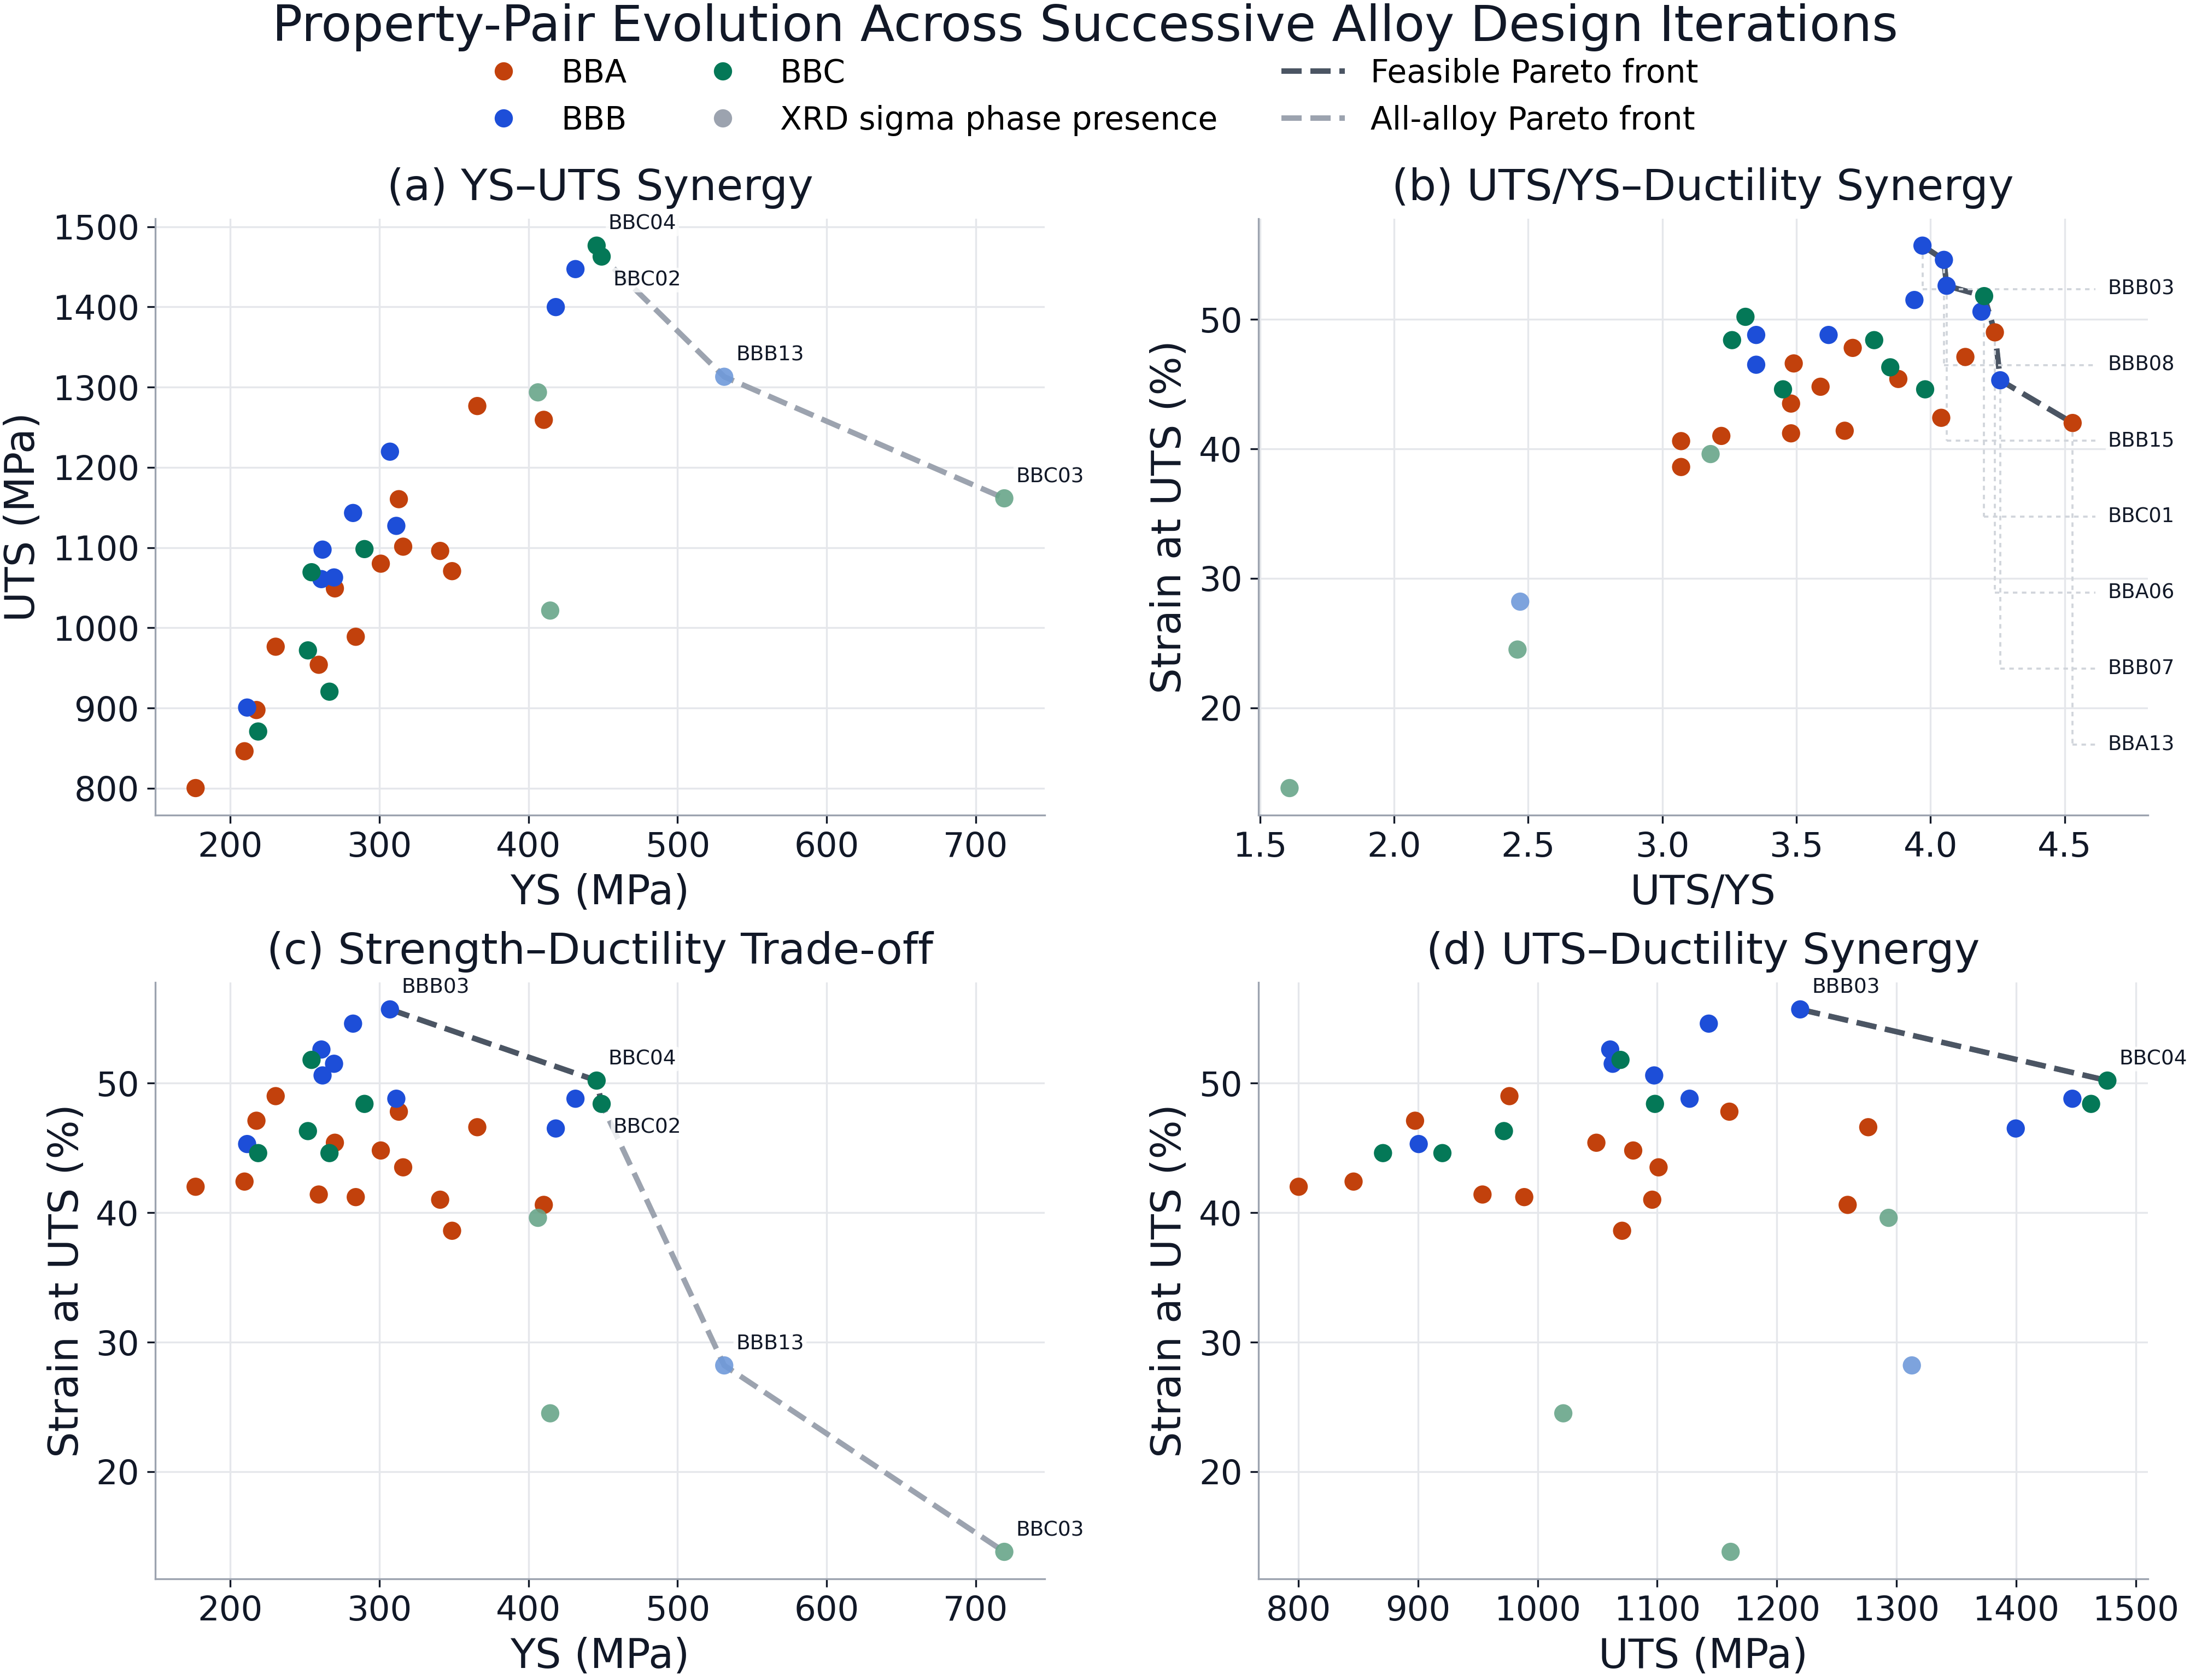
\includegraphics[width=0.8\linewidth]{Figures/pair_plots.png}
    \caption{Pair plots of mechanical property combinations across three successive design iterations. In each panel, solid arrows indicate the target direction for simultaneous property maximization, and dashed purple lines connect the best performing alloys for the given property pair. Labels identify individual alloy compositions discussed in the text.}
    \label{fig:pair_plots}
\end{figure}

\autoref{fig:pair_plots} shows four property--property relationships across the three design iterations. Panel~(a) shows yield strength versus ultimate tensile strength. Iteration~0 alloys (orange) cluster below ${\sim}350$~MPa yield strength and ${\sim}1100$~MPa UTS. Successive iterations progressively push the properties toward the upper-right region of this space: BBC04 reaches ${\sim}450$~MPa~YS at ${\sim}1450$~MPa~UTS, and BBB13 achieves ${\sim}530$~MPa~YS at ${\sim}1300$~MPa~UTS. BBC03 attains the highest yield strength (${\sim}720$~MPa) but at a comparatively lower UTS (${\sim}1100$~MPa), consistent with the embrittling effect of its secondary sigma phase. Panel~(b) plots tensile elongation against the UTS/YS ratio. A high UTS/YS ratio reflects substantial strain-hardening capacity, which enables greater uniform elongation. The best-performing alloys from Iterations~1 and~2 (BBB03, BBB08, BBB15, BBC01, and BBA06) cluster at elongations above 45\% with UTS/YS ratios exceeding 3.5, confirming that the optimization identified compositions with both high ductility and high work-hardening capacity. 

Panel~(c) directly visualizes the classical strength--ductility trade-off: elongation versus yield strength. The population follows a negative trend, with higher strength alloys exhibiting reduced elongation. Several later-iteration alloys approach this high strength, high ductility regime: BBC04 and BBC02 reach yield strengths of ${\sim}450$--490~MPa while maintaining elongations near 48--50\%, placing them above the overall trend. BBC03, by contrast, achieves ${\sim}720$~MPa yield strength at only ${\sim}14\%$ elongation, owing to the presence of sigma phase, making phase stability
a necessary design constraint.

Panel~(d) presents elongation versus UTS. Unlike panel~(c), the overall population shows no clear monotonic trend, because two competing mechanisms coexist: alloys that gain UTS at the expense of elongation, and alloys that achieve higher UTS through strain hardening without sacrificing ductility. Later iterations increasingly populate the latter category. BBB03 achieves ${\sim}1200$~MPa UTS at ${\sim}56\%$ elongation, while BBC04 combines the highest UTS in the dataset (${\sim}1480$~MPa) with elongation near 50\%. The progressive shift of Iteration~1 and~2 alloys into the upper-right quadrant provides direct evidence that the multi-objective optimization is successfully navigating the strength--ductility trade-off.

Collectively, these property relationships confirm advancement toward simultaneous maximization of strength and ductility in closed loop iterative alloy discovery. The underlying trade-off persists, most visibly in panel~(c), but the BIRDSHOT framework progressively identifies single phase FCC compositions that relax this constraint, expanding the accessible property space. The sigma bearing
alloys BBC03 and BBB13 serve as instructive counterexamples: their elevated yield strength comes at a steep ductility cost, signifying the importance of maintaining phase stability within the multi-objective design loop. A detailed analysis of these findings, including the compositional and microstructural factors of the observed improvement, will be presented in a forthcoming publication.                  


\subsubsection{Strength-Based correlations}

The relationship between material strength properties and ballistic resistance exhibited the expected inverse correlation, as illustrated in Figure~\ref{fig:DOPvAllStrengths}. The intuitive relationship between material strength and penetration resistance was confirmed through the simulation results. High-strength materials demonstrated superior penetration resistance due to their high resistance to deformation, yielding lower depth of penetration values when impacted. In contrast, low-strength materials exhibited higher DOP values under identical impact conditions.
Figure~\ref{fig:DOPvAllStrengths} (a) shows the clear negative correlation between DOP and yield strength, indicating that alloys with higher yield strengths provide enhanced ballistic protection. The ultimate tensile strength analysis (Figure~\ref{fig:DOPvAllStrengths}(b)) reinforced this relationship, showing that materials capable of withstanding higher ultimate loads before failure offer superior penetration resistance. The comprehensive strength properties analysis (Figure~\ref{fig:DOPvAllStrengths} provided an integrated view of how multiple strength parameters collectively influence ballistic performance, confirming the fundamental principle that stronger materials provide better ballistic protection.


\begin{figure}[H]
    \centering
    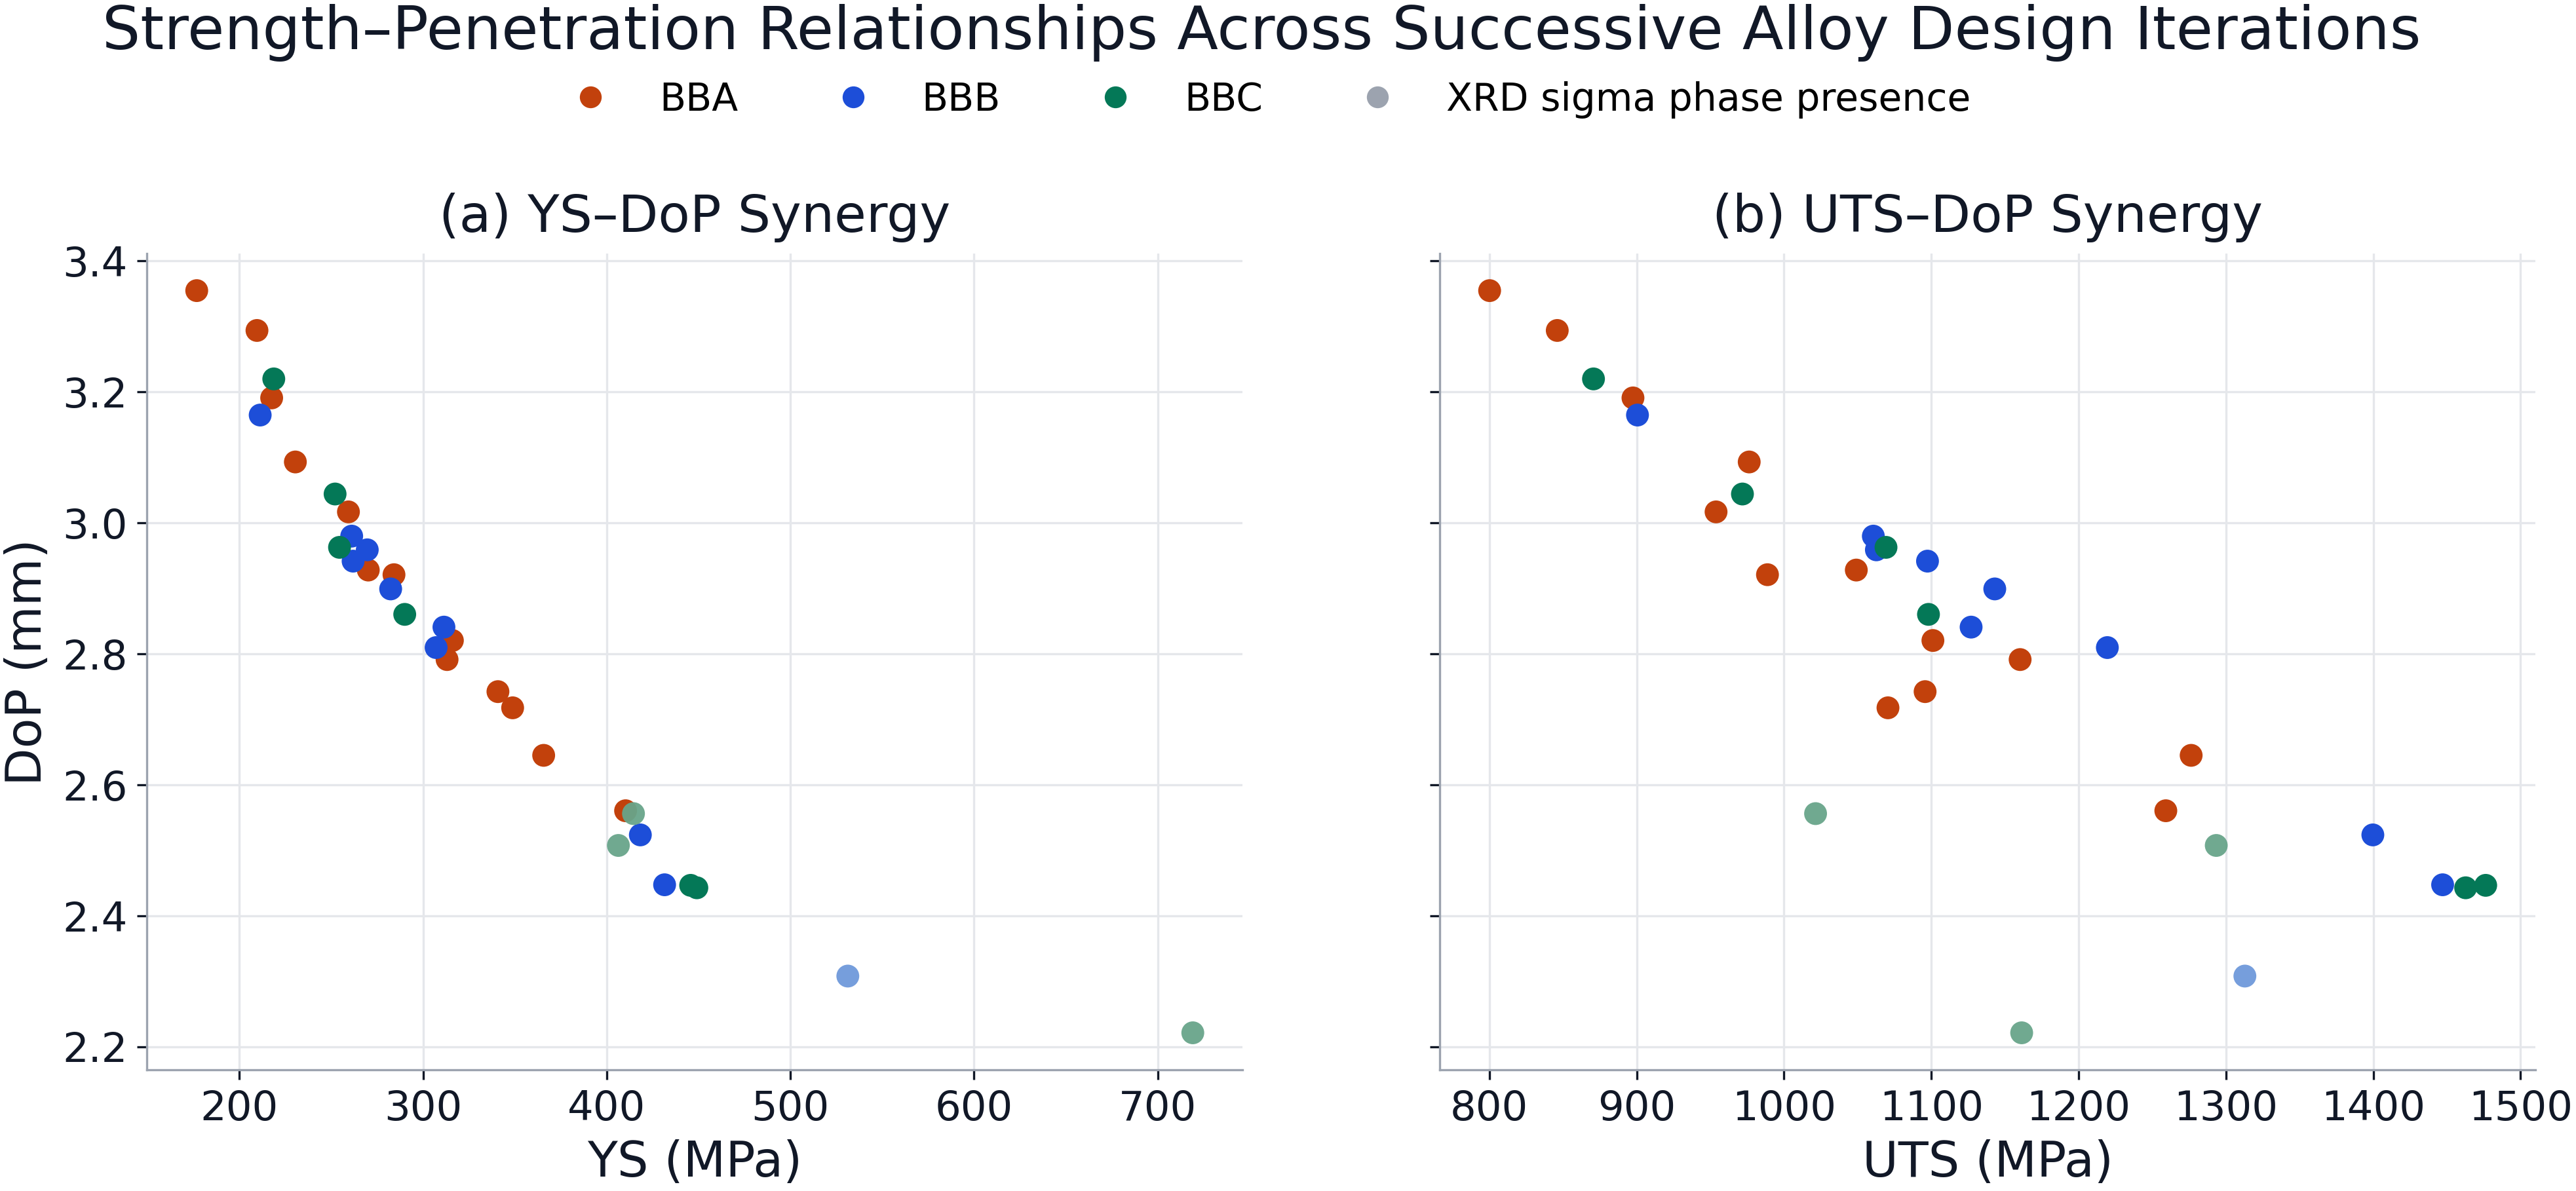
\includegraphics[width=0.8\linewidth]{Figures/Dop_vs_Strengths.png}
    \caption{Simulated depth of penetration (DOP) of projectiles into HEA targets as a function of quasi-static strength metrics across tested alloys.}
    \label{fig:DOPvAllStrengths}
\end{figure}

\subsubsection{Rate sensitivity analysis}
A notable finding from the analysis of DOP versus the calibrated rate-sensitivity exponent (\textit{M}) is presented in Figure~\ref{fig:DOPvM}. Surprisingly, there appeared to be little to no correlation between DOP and the rate-sensitivity parameter \textit{M}. However, the best performing alloys consistently exhibited calibrated \textit{M} values between 2 and 7, suggesting an optimal range for rate sensitivity in ballistic applications.
This relationship was further explored through the strength properties versus rate sensitivity analysis (Figure~\ref{fig:StrengthvM}). The alloy yield strength and ultimate tensile strength displayed negative correlations with \textit{M}, indicating that as the rate sensitivity exponent increases, the material strengths decrease. This inverse relationship suggests a fundamental trade-off in HEA design between rate sensitivity and quasi-static strength properties, highlighting the complex interplay between dynamic and static material behaviors.


\begin{figure}[H]
    \centering
    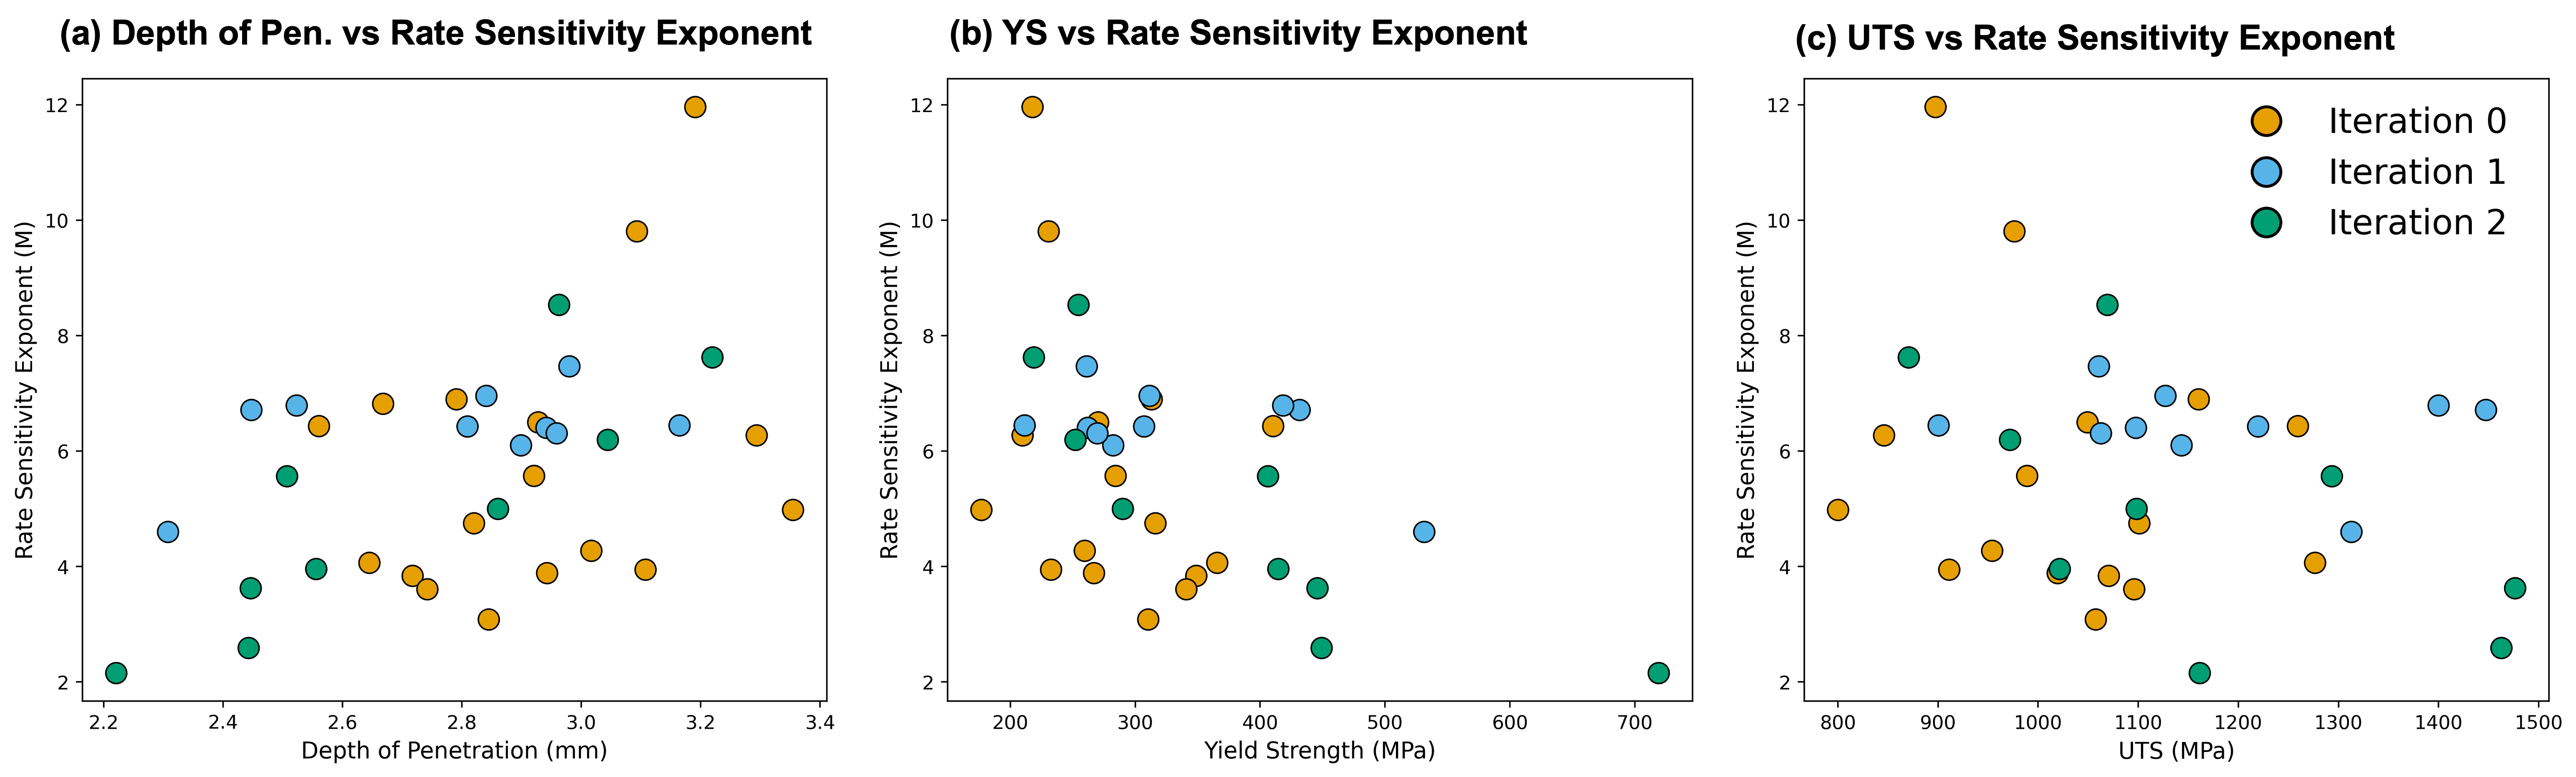
\includegraphics[width=0.9\linewidth]{Figures/M_plots.png}
    \caption{Rate sensitivity exponent (\textit{M}) as a function of key ballistic and mechanical properties for all candidate alloys across three iterations. (a) Simulated DOP of projectile on HEA target with respect to the calibrated rate-sensitivity exponent (\textit{M}) for each alloy. (b, c) Yield strength and ultimate tensile strength (UTS) versus \textit{M}, respectively.}
    \label{fig:MRelationships}
\end{figure}

Overall, these results reinforce the utility of DoP simulations as a scalable metric for high-rate performance screening. The strong alignment between strength and penetration resistance confirms that mechanical property data can serve as reliable predictors in the design process. Additionally, the parametric trends from synthetic modeling provide insight into how target properties may be tuned for future alloy development. Ongoing work will expand the parameter space and explore more advanced damage and failure criteria to further enhance predictive fidelity.


\subsection{Risk-Aware Bayesian Alloy Discovery and Findings}


In this study, substantial progress was made in accelerating the discovery of high performance HEAs for extreme environments, particularly high strain rate applications. The integrated framework, combining high-throughput synthesis, experimental automation, Bayesian optimization, and simulation-driven design, was rigorously validated through iterative alloy development. This study demonstrated that the design pipeline could not only generate structurally sound alloys across a vast chemical space but also systematically improve mechanical and ballistic performance across design iterations.

Across multiple acquisition iterations (BBA $\rightarrow$ BBB $\rightarrow$ BBC), the framework successfully produced candidate alloys with progressive improvements in both simulated and measured properties, validating the approach.

Table~\ref{tab:bo_metrics} summarizes the performance of the Bayesian optimization framework across successive acquisition iterations demonstrating substantial progress in the same. Beginning with iteration BBA, the initial Pareto front contained 10 non-dominated alloys with a hypervolume of 658.24. Upon incorporating mechanical test results and simulated depth of penetration data, the next batch of candidates (BBB) showed a remarkable 27.1\% gain in average Expected Hypervolume Improvement, increasing the true hypervolume to 817.77. The number of Pareto-optimal alloys also rose to 17, with 9 new entries contributed by iteration BBB alone, demonstrating the algorithm's success in identifying diverse high-performance solutions.

In the following iteration (BBC), the framework continued this upward trend, yielding a 27.2\% increase in EHVI and reaching a new hypervolume of 856.30. The Pareto front expanded to 21 compositions, with 5 additional new entries contributed by iteration BBC. These consistent improvement rates indicate effective learning, exploration, and exploitation of the design space, with the algorithm successfully balancing exploration of uncertain regions with exploitation of identified high-performance zones. The steady 27\% improvement rates observed between iterations suggest that the Bayesian optimization framework maintained effective learning throughout the study without premature convergence.

\begin{table}[H]
\centering
\caption{Bayesian Optimization Performance Across Iterations}
\label{tab:bo_metrics}
\begin{tabular}{lccc}
\toprule
\textbf{Iteration} & \textbf{Avg EHVI} & \textbf{Hypervolume (HV)} & \textbf{Pareto Front Size} \\
\midrule
BBA & N/A & 658.24 & 10 \\
BBB & 836.41 (27.1\%) & 817.77 & 17 (9 new) \\
BBC & 1059.2 (27.2\%) & 856.30 & 21 (5 new) \\
\bottomrule
\end{tabular}
\end{table}


The combination of mechanical property measurements (YS, UTS/YS, strain at UTS), rate sensitivity metrics (from SHPB and nanoindentation), and simulated impact resistance (via DoP modeling) enabled a multi-modal assessment of each candidate alloy. The optimization framework consistently identified alloys that offered superior performance in at least one or more of the objectives, while preserving chemical diversity across the 37 subsystems. Notably, many top-performing alloys from later iterations (e.g., BBB13, BBC03) showed improved dynamic hardness and reduced DoP, validating the use of surrogate models trained on early experimental data.



\emph{Risk-Aware Decision Making}

The risk-aware nature of the Bayesian optimization framework proved valuable in the current study. By incorporating uncertainty quantification into the acquisition function, the algorithm avoided over-exploitation of potentially misleading high-performance predictions while ensuring exploration of the compositional space. This approach is particularly critical for applications where material failure can have catastrophic consequences.

The expected hypervolume improvement criterion inherently accounts for uncertainty in both the predictive models and the multi-objective trade-offs, providing a mathematically rigorous approach to risk-aware materials discovery. The consistent performance improvements observed across iterations validate this risk-aware strategy's effectiveness in identifying reliable high-performance compositions. This approach is particularly critical for functional applications where material reliability is critical and over-exploitation of potentially misleading predictions must be avoided.


The results demonstrate that the BO framework is capable of progressively refining alloy selection, increasing solution quality, and expanding the Pareto front over time. The observed improvements in both performance metrics and diversity validate the utility of an integrated machine learning, simulation, and experimental workflow for high-throughput alloy discovery.


From a broader perspective, these results validate the scalability and adaptability of the integrated materials discovery framework. The iterative optimization not only improved alloy performance metrics but also reinforced the potential of closed-loop AI/ML-driven design in navigating complex, high-dimensional material spaces.

\subsection{Property and Performance Evolution Visualizations}

The comprehensive visualization analysis results in this study provide detailed insights into the multi-dimensional relationships between material properties and performance metrics across the iterations. The visualization suite, consisting of pairplots and boxplots, reveals complex correlations and optimization trajectories that validate the effectiveness of the risk-aware discovery framework.

% \emph{Property Correlation Analysis}

% The pairplot analysis in \autoref{fig:pairplot_correlations} reveals relationships between the performance metrics: dynamic hardness (Hdyn), quasi-static hardness (Hqs), hardness ratio (Hdyn/Hqs), yield strength (YS), ultimate tensile strength (UTS), strain at UTS, strength ratio (UTS/YS), and penetration depth. The diagonal elements of the pairplot matrix show the distribution characteristics of each property, while the off-diagonal scatter plots illuminate pairwise correlations that are critical for understanding multi-objective optimization.

% \begin{figure}[H]
%     \centering
%     \includegraphics[width=0.9\linewidth]{Figures/Property_Pair_Plot.png}
%     \caption{Comprehensive pairwise analysis of mechanical and ballistic properties for HEAs across all iterations within the study. Data points are color-coded by iteration: BBA (orange), BBB (blue), and BBC (green)}
%     \label{fig:pairplot_correlations}
% \end{figure}


% Strong positive correlations are observed between strength-related properties (YS, UTS, Hdyn, Hqs), indicating that the optimization framework successfully identified compositional regions where multiple strength metrics improve simultaneously. This finding is particularly significant as it demonstrates that the high entropy alloy system enables concurrent enhancement of seemingly independent mechanical properties, challenging traditional materials design paradigms that often assume trade-offs between different strength measures.

% The correlation between dynamic and quasi-static properties reveals important insights for strain rate sensitive applications. The positive correlation between Hdyn and Hqs suggests fundamental material hardness improvements, while the distribution of Hdyn/Hqs ratios indicates varying degrees of strain-rate sensitivity across the alloy compositions. Alloys exhibiting higher Hdyn/Hqs ratios represent compositions that are particularly well-suited for high strain-rate applications such as ballistic protection.


\emph{Statistical Distribution Evolution}

The box plot analysis in \autoref{fig:boxplot_properties} provides statistical insights into the evolution of property distributions across optimization iterations, showing improvements and changes in variability. The progression from BBA through BBC iterations shows consistent improvements in median values for strength-related properties (YS, UTS, Hdyn, Hqs) while simultaneously reducing inter-quartile ranges, indicating convergence toward more consistent high-performance compositions.

\begin{figure}[H]
    \centering
    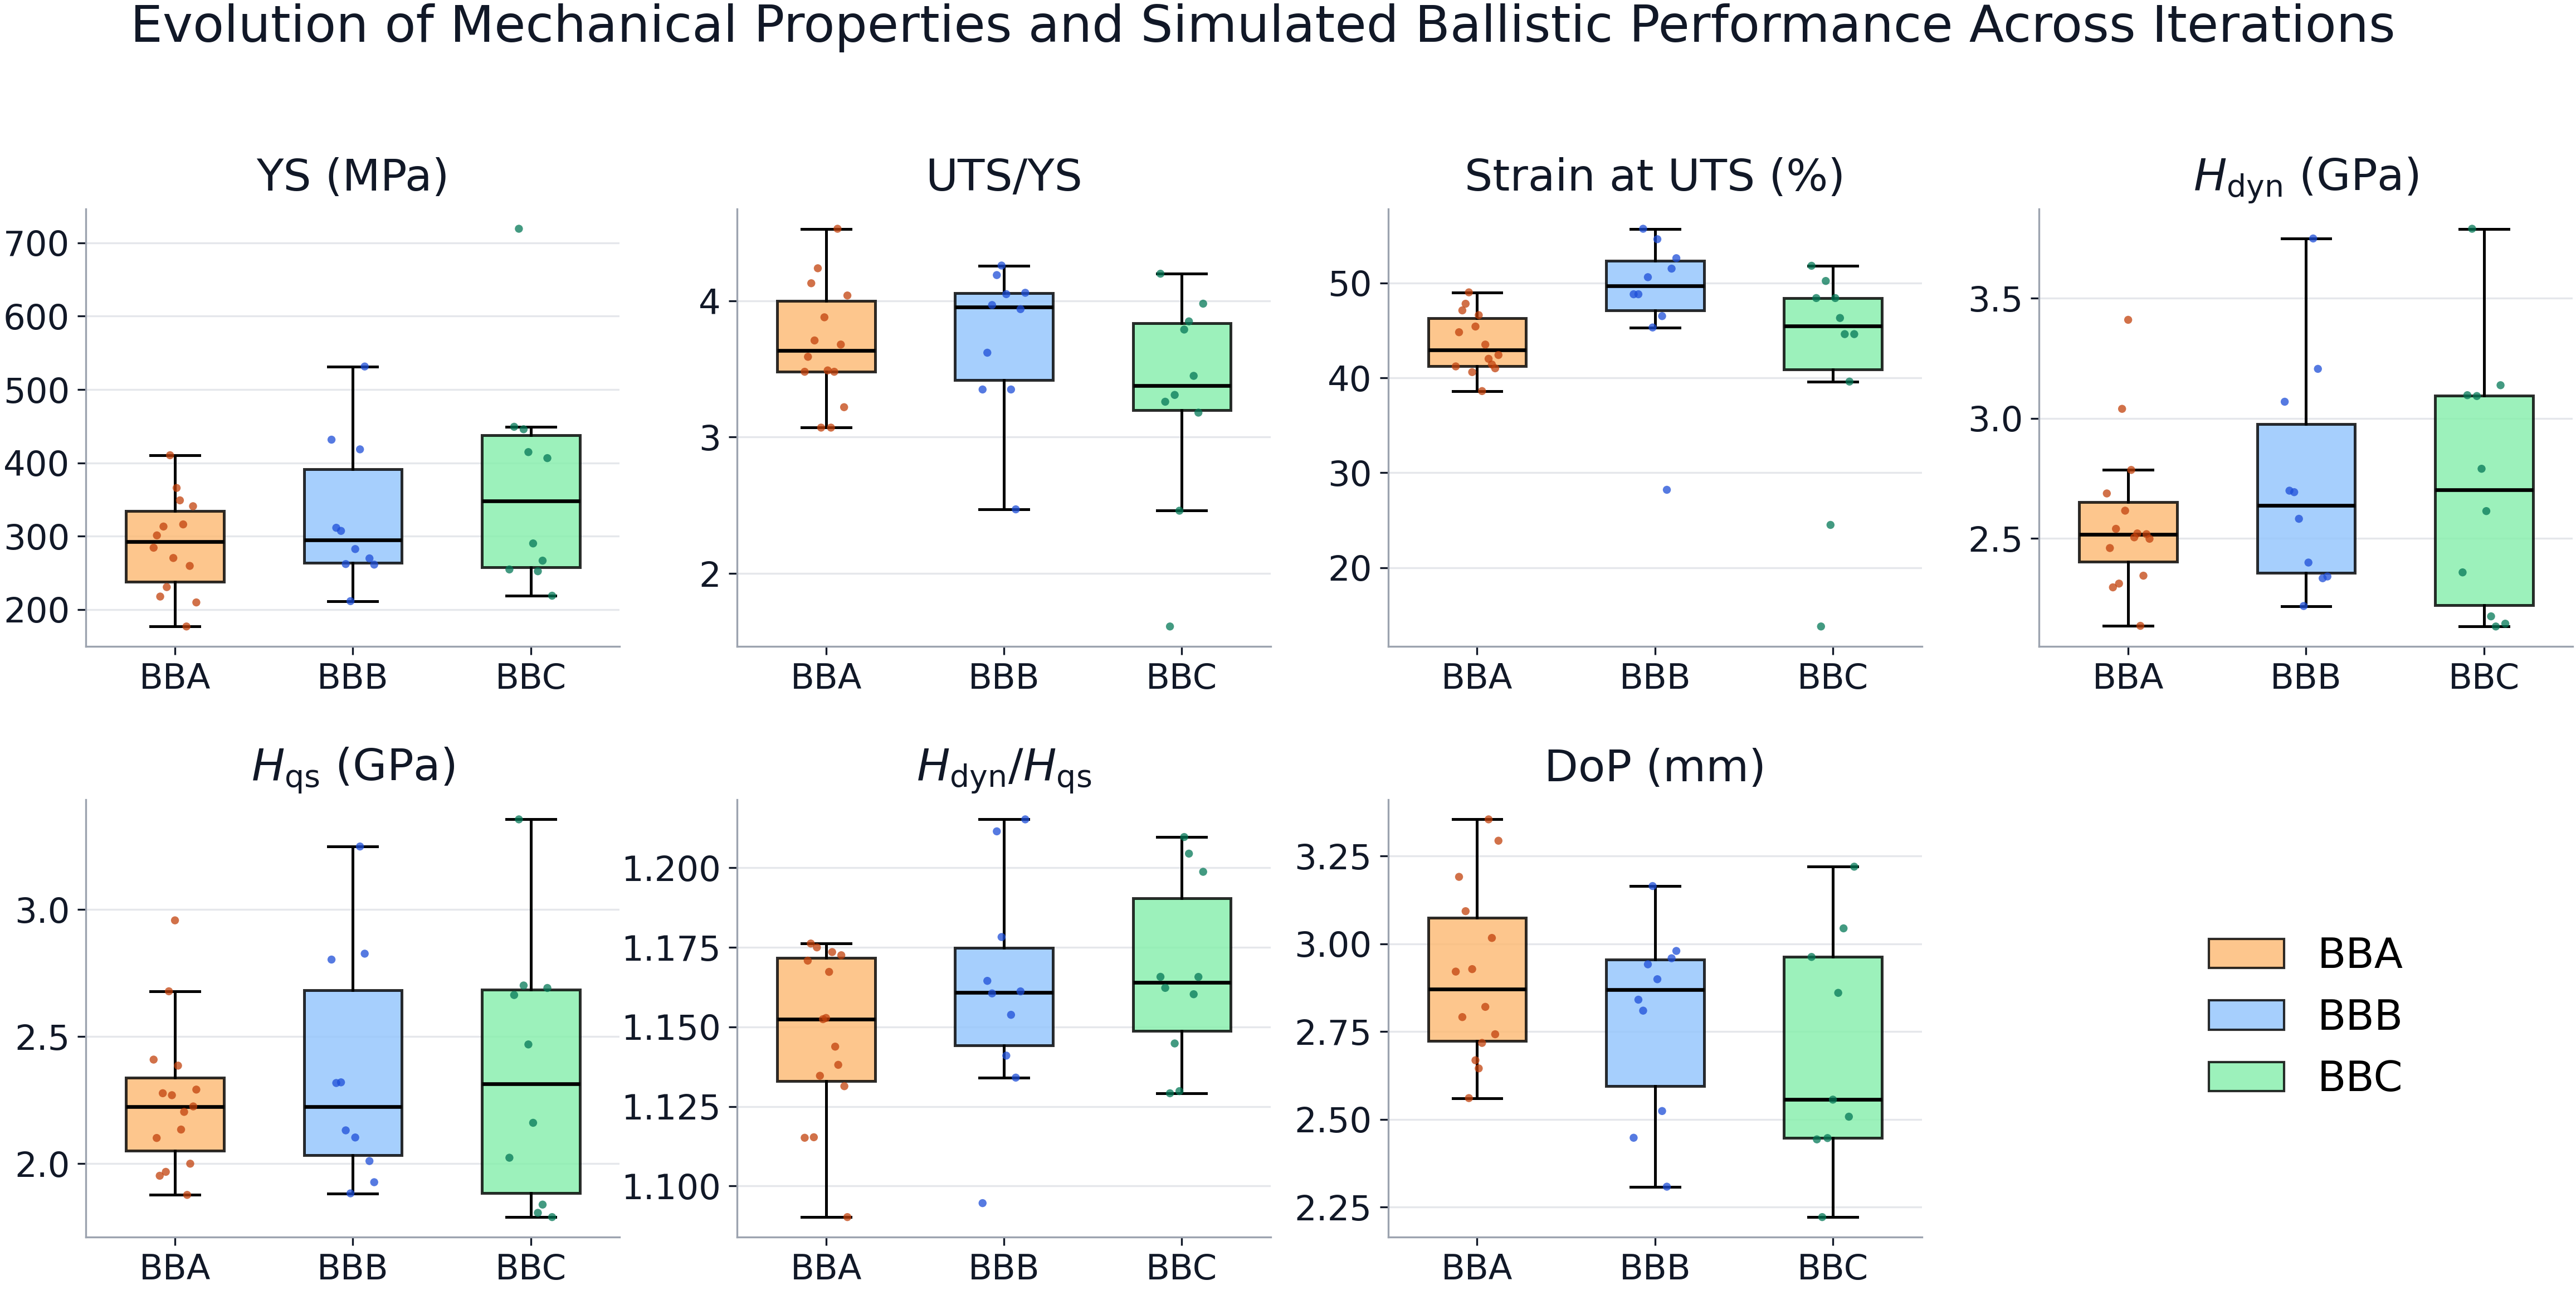
\includegraphics[width=0.9\linewidth]{Figures/box_plot.png}
    \caption{Boxplot analysis showing the evolution of mechanical properties and ballistic performance across all iterations. The progression from BBA (baseline) to BBC iterations demonstrates systematic improvement in strength properties, strain-rate sensitivity, ductility, and ballistic resistance. Color coding: orange (BBA), blue (BBB), green (BBC).}
    \label{fig:boxplot_properties}
\end{figure}

The penetration depth boxplot results show a noteworthy trend, with median values decreasing across iterations while the distribution becomes more tightly clustered around lower penetration depths. %This dual improvement—better average performance and reduced variability—is critical for ballistic protection applications where both high performance and reliability are essential requirements.
The strain at UTS distributions reveal interesting optimization dynamics, showing maintained or improved ductility characteristics despite significant strength enhancements. This preservation of ductility while achieving higher strength levels demonstrates the unique advantages of the high entropy alloy system and the effectiveness of the multi-objective optimization approach in avoiding traditional strength-ductility trade-offs.

The visualization results also validate the multi-fidelity approach employed in the optimization framework, where high-fidelity experimental data (tension tests for yield strength) are combined with lower-fidelity measurements (indentation tests for dynamic properties) and simulations (finite element analysis for penetration depth). The coherent improvement patterns observed across all fidelity levels demonstrate the effectiveness of this integrated approach.

